% Capitolul 3: Modele ARIMA pentru Date Nestaționare
% Prezentare academică de calitate Harvard
% Program de licență, Academia de Studii Economice din București

\documentclass[9pt, aspectratio=169, t]{beamer}

% Asigură încadrarea conținutului pe diapozitive
\setbeamersize{text margin left=8mm, text margin right=8mm}

%=============================================================================
% CONFIGURARE TEMĂ ȘI STIL
%=============================================================================
\usetheme{default}
% Utilizăm tema implicită pentru control curat al antetului/subsolului

% Paletă de Culori (potrivită cu PDF-ul Redispatch)
\definecolor{MainBlue}{RGB}{26, 58, 110}
\definecolor{AccentBlue}{RGB}{26, 58, 110}
\definecolor{IDAred}{RGB}{205, 0, 0}
\definecolor{DarkGray}{RGB}{51, 51, 51}
\definecolor{MediumGray}{RGB}{128, 128, 128}
\definecolor{LightGray}{RGB}{248, 248, 248}
\definecolor{VeryLightGray}{RGB}{235, 235, 235}
\definecolor{KeynoteGray}{RGB}{218, 218, 218}
\definecolor{SectionGray}{RGB}{120, 120, 120}
\definecolor{FooterGray}{RGB}{100, 100, 100}
\definecolor{Crimson}{RGB}{220, 53, 69}
\definecolor{Forest}{RGB}{46, 125, 50}
\definecolor{Amber}{RGB}{181, 133, 63}
\definecolor{Orange}{RGB}{230, 126, 34}
\definecolor{Purple}{RGB}{142, 68, 173}

% Fundal gradient (gradient Keynote exact 315°: alb la RGB 218,218,218)
\setbeamertemplate{background}{%
    \begin{tikzpicture}[remember picture, overlay]
        \shade[shading=axis, shading angle=315,
        top color=white, bottom color=KeynoteGray]
        (current page.south west) rectangle (current page.north east);
    \end{tikzpicture}%
}
% Culoare solidă de rezervă pentru compatibilitate
\setbeamercolor{background canvas}{bg=}

\setbeamercolor{palette primary}{bg=MainBlue, fg=white}
\setbeamercolor{palette secondary}{bg=MainBlue!85, fg=white}
\setbeamercolor{palette tertiary}{bg=MainBlue!70, fg=white}
\setbeamercolor{structure}{fg=MainBlue}
\setbeamercolor{title}{fg=IDAred}
\setbeamercolor{frametitle}{fg=IDAred, bg=}
\setbeamercolor{block title}{bg=MainBlue, fg=white}
\setbeamercolor{block body}{bg=VeryLightGray, fg=DarkGray}
\setbeamercolor{block title alerted}{bg=Crimson, fg=white}
\setbeamercolor{block body alerted}{bg=Crimson!8, fg=DarkGray}
\setbeamercolor{block title example}{bg=Forest, fg=white}
\setbeamercolor{block body example}{bg=Forest!8, fg=DarkGray}
\setbeamercolor{item}{fg=MainBlue}

% Culori subsol (suprascriu albastrul temei Madrid)
\setbeamercolor{author in head/foot}{fg=FooterGray, bg=}
\setbeamercolor{title in head/foot}{fg=FooterGray, bg=}
\setbeamercolor{date in head/foot}{fg=FooterGray, bg=}
\setbeamercolor{section in head/foot}{fg=FooterGray, bg=}
\setbeamercolor{subsection in head/foot}{fg=FooterGray, bg=}

% Stiluri marcatori (se aplică peste tot inclusiv în blocuri)
\setbeamertemplate{itemize item}{\color{MainBlue}$\boxdot$}
\setbeamertemplate{itemize subitem}{\color{MainBlue}$\blacktriangleright$}
\setbeamertemplate{itemize subsubitem}{\color{MainBlue}\tiny$\bullet$}
\setbeamertemplate{itemize/enumerate body begin}{\normalsize}
\setbeamertemplate{itemize/enumerate subbody begin}{\normalsize}

% Item spacing - compact style
\setlength{\leftmargini}{10pt}       % Level 1: minimal indent
\setlength{\leftmarginii}{10pt}      % Level 2: minimal additional indent
% Compact list spacing (zero extra space before/after lists in blocks)
\makeatletter
\def\@listi{\leftmargin\leftmargini \topsep 0pt \parsep 0pt \itemsep 0pt}
\def\@listii{\leftmargin\leftmarginii \topsep 0pt \parsep 0pt \itemsep 0pt}
\makeatother

\setbeamertemplate{navigation symbols}{}

%=============================================================================
% ANTET PERSONALIZAT
%=============================================================================
\setbeamertemplate{headline}{%
    \vskip10pt%
    \hbox to \paperwidth{%
        \hskip0.5cm%
        {\small\color{FooterGray}\renewcommand{\hyperlink}[2]{##2}\insertsectionhead}%
        \hfill%
        \textcolor{FooterGray}{\small\insertframenumber}%
        \hskip0.5cm%
    }%
    \vskip4pt%
    {\color{FooterGray}\hrule height 0.4pt}%
}

%=============================================================================
% CUSTOM FOOTER
%=============================================================================
\usepackage{fontawesome5}

\setbeamertemplate{footline}{%
    {\color{FooterGray}\hrule height 0.4pt}%
    \vskip4pt%
    \hbox to \paperwidth{%
        \hskip0.5cm%
        \textcolor{FooterGray}{\small Analiza și Prognoza Seriilor de Timp}%
        \hfill%
        \raisebox{-0.1em}{%
            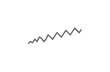
\begin{tikzpicture}[x=0.08em, y=0.08em, line width=0.4pt]
                \draw[FooterGray] (0,3) -- (1,4) -- (2,3.5) -- (3,5) -- (4,4) -- (5,6) -- (6,5.5) -- (7,4) -- (8,5) -- (9,7) -- (10,6) -- (11,5) -- (12,6.5) -- (13,8) -- (14,7) -- (15,6) -- (16,7.5) -- (17,9) -- (18,8) -- (19,7) -- (20,8.5) -- (21,10) -- (22,9) -- (23,8) -- (24,9.5);
            \end{tikzpicture}%
        }%
        \hskip0.5cm%
    }%
    \vskip6pt%
}

%=============================================================================
% PACHETE
%=============================================================================
\usepackage[utf8]{inputenc}
\usepackage[T1]{fontenc}
\usepackage{amsmath, amssymb, amsthm}
\usepackage{mathtools}
\usepackage{bm}
\usepackage{tikz}
\usetikzlibrary{arrows.meta, positioning, shapes, calc, decorations.pathreplacing, shadings}
\usepackage{booktabs}
\usepackage{multirow}
\usepackage{array}
\usepackage{graphicx}
\usepackage{hyperref}
\usepackage{colortbl}
\hypersetup{colorlinks=true, linkcolor=MainBlue, urlcolor=MainBlue}
\graphicspath{{../../logos/}{../../charts/}{../../photos/}}
\hfuzz=2pt  % Suppress tiny overfull warnings (<2pt)
\vfuzz=2pt  % Suppress tiny vertical overfull warnings (<2pt)

%=============================================================================
% COMANDA QUANTLET
%=============================================================================
\newcommand{\quantlet}[2]{%
    \hfill\href{#2}{%
        \raisebox{-0.15em}{\includegraphics[height=0.7em]{ql_logo.png}}%
        \textcolor{MainBlue}{\tiny\ #1}%
    }%
}

%=============================================================================
% MEDII PENTRU TEOREME
%=============================================================================
\theoremstyle{definition}
\setbeamertemplate{theorems}[numbered]
\newtheorem{defn}{Definiție}
\newtheorem{thm}{Teoremă}
\newtheorem{prop}{Propoziție}
\newtheorem{rmk}{Observație}

%=============================================================================
%=============================================================================
% CENTRED MINIPAGE (fara spatiu vertical suplimentar)
%=============================================================================
\newenvironment{cminipage}[1]{%
    \par\noindent\hfill\begin{minipage}{#1}\ignorespaces
}{%
    \end{minipage}\hfill\null\par
}


% COMENZI PERSONALIZATE
%=============================================================================
\newcommand{\E}{\mathbb{E}}
\newcommand{\Var}{\text{Var}}
\newcommand{\Cov}{\text{Cov}}
\newcommand{\Corr}{\text{Corr}}
\newcommand{\R}{\mathbb{R}}
\newcommand{\N}{\mathbb{N}}
\newcommand{\Z}{\mathbb{Z}}
\newcommand{\B}{\mathbf{B}}
\newcommand{\imark}{\textcolor{MainBlue}{\textbullet}}
\newcommand{\RMSE}{\text{RMSE}}
\newcommand{\MAE}{\text{MAE}}
\newcommand{\MAPE}{\text{MAPE}}

%=============================================================================
% PAGINĂ TITLU PERSONALIZATĂ
%=============================================================================
\defbeamertemplate*{title page}{hybrid}[1][]
{
    \vspace{0.2cm}
    % Rând logo-uri - antet superior (cu linkuri clickabile)
    \begin{center}
        \href{https://www.ase.ro}{\includegraphics[height=1.0cm]{ase_logo.png}}\hspace{0.3cm}%
        \href{https://theida.net}{\includegraphics[height=1.0cm]{ida_logo.png}}\hspace{0.3cm}%
        \href{https://blockchain-research-center.com}{\includegraphics[height=1.0cm]{brc_logo.png}}\hspace{0.3cm}%
        \href{https://www.ai4efin.ase.ro}{\includegraphics[height=1.0cm]{ai4efin_logo.png}}\hspace{0.3cm}%
        \href{https://ipe.ro/new}{\includegraphics[height=1.0cm]{acad_logo.png}}\hspace{0.3cm}%
        \href{https://www.digital-finance-msca.com}{\includegraphics[height=1.0cm]{msca_logo.png}}%
    \end{center}

    \vspace{0.6cm}

    % Titlu principal cu logo-uri Q pe părți (cu linkuri clickabile)
    \begin{center}
        \begin{minipage}{0.1\textwidth}
            \centering
            \href{https://quantlet.com}{\includegraphics[height=1.1cm]{ql_logo.png}}
        \end{minipage}%
        \begin{minipage}{0.78\textwidth}
            \centering
            {\LARGE\bfseries\usebeamercolor[fg]{title}\inserttitle}

            \vspace{0.3cm}

            {\usebeamerfont{subtitle}\usebeamercolor[fg]{title}\insertsubtitle}
        \end{minipage}%
        \begin{minipage}{0.1\textwidth}
            \centering
            \href{https://quantinar.com}{\includegraphics[height=1.1cm]{qr_logo.png}}
        \end{minipage}
    \end{center}

    \vspace{0.6cm}

    % Autori (aliniere la stânga)
    \hspace{0.5cm}{\usebeamerfont{author}\insertauthor}

    \vspace{0.3cm}

    % Institut/Afilieri (aliniere la stânga)
    \hspace{0.5cm}\begin{minipage}[t]{0.9\textwidth}
        \raggedright\small\insertinstitute
    \end{minipage}
}

%=============================================================================
% INFORMAȚII TITLU
%=============================================================================
\title[Analiza Seriilor de Timp]{Analiza și Prognoza Seriilor de Timp}
\subtitle{Capitolul 3: Modele ARIMA pentru Date Nestaționare}
\author[D.T. Pele]{Daniel Traian PELE}
\institute{Academia de Studii Economice din București\\
IDA Institute Digital Assets\\
Blockchain Research Center\\
AI4EFin Artificial Intelligence for Energy Finance\\
Academia Română, Institutul de Prognoză Economică\\
MSCA Digital Finance}
\date{}

\begin{document}

% Pagina de titlu (fără antet/subsol)
{
\setbeamertemplate{headline}{}
\setbeamertemplate{footline}{}
\begin{frame}
    \titlepage
\end{frame}
}

%=============================================================================
% OBIECTIVE DE ÎNVĂȚARE
%=============================================================================
\begin{frame}{Obiective de Învățare}
    \begin{cminipage}{0.95\textwidth}
    {\small
    \begin{block}{La finalul acestui capitol, veți fi capabili să:}
    \begin{enumerate}\setlength{\itemsep}{0pt}
        \item[\textcolor{MainBlue}{\textbf{1.}}] \textbf{Înțelegeți} conceptul de nestaționaritate și implicațiile sale
        \item[\textcolor{MainBlue}{\textbf{2.}}] \textbf{Aplicați} diferențierea pentru a obține staționaritate
        \item[\textcolor{MainBlue}{\textbf{3.}}] \textbf{Folosiți} testul Augmented Dickey-Fuller (ADF) pentru detectarea rădăcinii unitate
        \item[\textcolor{MainBlue}{\textbf{4.}}] \textbf{Construiți}, estimați și prognozați cu modele ARIMA($p,d,q$)
        \item[\textcolor{MainBlue}{\textbf{5.}}] \textbf{Evaluați} prognozele prin metoda ferestrei rolling
        \item[\textcolor{MainBlue}{\textbf{6.}}] \textbf{Aplicați} metodologia Box-Jenkins pe date reale (PIB SUA)
    \end{enumerate}
    \end{block}
    }
    \end{cminipage}
\end{frame}

%=============================================================================
% SURSE DE DATE ȘI INSTRUMENTE SOFTWARE
%=============================================================================
\begin{frame}{Surse de date și instrumente software}
    \begin{cminipage}{0.95\textwidth}
    \begin{columns}[T]
        \begin{column}{0.48\textwidth}
            \begin{block}{Surse de date}
                \begin{itemize}\setlength{\itemsep}{0pt}
                    \item \textbf{FRED} (Federal Reserve)
                    \begin{itemize}
                        \item PIB real SUA (GDPC1), rate dobânzi
                    \end{itemize}
                    \item \textbf{Yahoo Finance}
                    \begin{itemize}
                        \item Prețuri acțiuni, cursuri de schimb
                    \end{itemize}
                    \item \textbf{Eurostat / BNR}
                    \begin{itemize}
                        \item Date macroeconomice europene
                    \end{itemize}
                    \item \textbf{Statsmodels datasets}
                    \begin{itemize}
                        \item Sunspots, Nile, Macrodata
                    \end{itemize}
                \end{itemize}
            \end{block}
        \end{column}
        \begin{column}{0.48\textwidth}
            \begin{exampleblock}{Python}
                \begin{itemize}\setlength{\itemsep}{0pt}
                    \item \texttt{statsmodels} --- modele ARIMA
                    \item \texttt{pmdarima} --- selecție automată
                    \item \texttt{pandas-datareader} --- descărcare FRED
                    \item \texttt{matplotlib} --- vizualizare
                    \item \texttt{scipy} --- teste statistice
                \end{itemize}
            \end{exampleblock}
            \begin{alertblock}{Resurse}
                \begin{itemize}\setlength{\itemsep}{0pt}
                    \item \href{https://github.com/QuantLet/TSA/tree/main/TSA_ch3}{\texttt{github.com/QuantLet/TSA/TSA\_ch3}}
                    \item \href{https://quantlet.com}{\texttt{quantlet.com}}
                \end{itemize}
            \end{alertblock}
        \end{column}
    \end{columns}
    \end{cminipage}
\end{frame}

%=============================================================================
% STRUCTURA CAPITOLULUI
%=============================================================================
\begin{frame}{Structura capitolului}
    \begin{cminipage}{0.95\textwidth}
    \setbeamertemplate{section in toc}{\color{MainBlue}$\boxdot$~\inserttocsection}
    \tableofcontents
    \end{cminipage}
\end{frame}

%=============================================================================
% MOTIVAȚIE
%=============================================================================
\section{Motivație}

\begin{frame}{De ce ARIMA? Datele nestaționare sunt pretutindeni}
    \begin{center}
        \includegraphics[width=0.95\textwidth, height=0.78\textheight, keepaspectratio]{ch3_motivation_nonstationary.pdf}
    \end{center}
    \quantlet{TSA\_ch3\_motivation\_nonstationary}{https://github.com/QuantLet/TSA/tree/main/TSA_ch3/TSA_ch3_motivation_nonstationary}
\end{frame}

\begin{frame}{De ce ARIMA? Datele nestaționare sunt pretutindeni}
    \vspace{-0.2cm}
    {\footnotesize
    \begin{exampleblock}{}
        \begin{itemize}\setlength{\itemsep}{0pt}
            \item Prețurile acțiunilor, PIB, cursurile de schimb prezintă \textbf{trenduri} sau \textbf{mers aleatoriu}
            \item Media din eșantion (linia roșie) este lipsită de sens pentru un mers aleator ($\bar{x} = \frac{1}{n}\sum_{i=1}^n x_i$)
            \item Modelele ARMA standard \textbf{nu pot} gestiona aceste serii direct
        \end{itemize}
    \end{exampleblock}
    }
\end{frame}

\begin{frame}{Aplicații practice}
    \begin{center}
        \includegraphics[width=0.95\textwidth, height=0.78\textheight, keepaspectratio]{ch3_motivation_realworld.pdf}
    \end{center}
    \quantlet{TSA\_ch3\_motivation\_realworld}{https://github.com/QuantLet/TSA/tree/main/TSA_ch3/TSA_ch3_motivation_realworld}
\end{frame}

\begin{frame}{Aplicații practice}
    \vspace{-0.2cm}
    \vspace{0.3cm}
    {\footnotesize
    \begin{alertblock}{Provocarea}
        \begin{itemize}\setlength{\itemsep}{2pt}
            \item Prețuri de acțiuni: mers aleator (preț logaritmic)
            \item Cursuri de schimb: mers aleator
            \item Rate ale dobânzii: foarte persistente, aproape de rădăcină unitate
        \end{itemize}
    \end{alertblock}
    }
\end{frame}

\begin{frame}{Soluția: diferențierea}
    \begin{center}
        \includegraphics[width=0.95\textwidth, height=0.78\textheight, keepaspectratio]{ch3_motivation_differencing.pdf}
    \end{center}
    \quantlet{TSA\_ch3\_motivation\_differencing}{https://github.com/QuantLet/TSA/tree/main/TSA_ch3/TSA_ch3_motivation_differencing}
\end{frame}

\begin{frame}{Soluția: diferențierea}
    \vspace{-0.2cm}
    {\footnotesize
    \begin{exampleblock}{Observație Cheie}
        \begin{itemize}\setlength{\itemsep}{0pt}
            \item \textbf{Diferențierea} transformă o serie nestaționară într-una staționară: $\Delta Y_t = Y_t - Y_{t-1}$
            \item ACF se schimbă de la descreștere lentă la descreștere rapidă!
        \end{itemize}
    \end{exampleblock}
    }
\end{frame}

\begin{frame}{Ce vom învăța astăzi}
    \begin{cminipage}{0.95\textwidth}
    \begin{block}{Concepte Fundamentale}
        \begin{enumerate}
            \item \textbf{Nestaționaritatea}: de ce contează și cum o detectăm
            \item \textbf{Teste de rădăcină unitate}: ADF, PP, KPSS
            \item \textbf{Diferențierea}: transformarea cheie
            \item \textbf{Modele ARIMA}: combinarea diferențierii cu ARMA
            \item \textbf{Metodologia Box-Jenkins}: Identificare $\to$ Estimare $\to$ Diagnoză
        \end{enumerate}
    \end{block}

    \vspace{0.2cm}

    \begin{exampleblock}{La Sfârșitul Acestui Curs}
        Veți putea modela și prognoza serii de timp nestaționare precum prețurile acțiunilor, PIB-ul și cursurile de schimb folosind modele ARIMA.
    \end{exampleblock}
    \end{cminipage}
\end{frame}

%=============================================================================
% SECȚIUNEA 1: NESTAȚIONARITATEA
%=============================================================================
\section{Nestaționaritatea în seriile de timp}

\begin{frame}{De ce contează nestaționaritatea}
    \begin{cminipage}{0.95\textwidth}
    {\small
    \begin{alertblock}{Problema}
        \begin{itemize}\setlength{\itemsep}{0pt}
            \item Multe serii de timp economice și financiare sunt \textbf{nestaționare}:
            \begin{itemize}\setlength{\itemsep}{0pt}
                \item PIB, prețuri de acțiuni, cursuri de schimb, indici de inflație
                \item Prezintă trenduri, medii în schimbare sau varianță în creștere
            \end{itemize}
        \end{itemize}
    \end{alertblock}

    \vspace{0.1cm}

    \begin{block}{Consecințele Nestaționarității}
        \begin{itemize}\setlength{\itemsep}{0pt}
            \item Modelele ARMA standard presupun staționaritate
            \item Regresia OLS cu date nestaționare duce la \textbf{regresie falsă}
            \item Momentele din eșantion (medie, varianță, ACF) nu sunt estimatori consistenți
            \item Inferența statistică devine invalidă
        \end{itemize}
    \end{block}
    }
    \end{cminipage}
\end{frame}

\begin{frame}{Exemplu: PIB real SUA}
    \begin{center}
        \includegraphics[width=0.95\textwidth, height=0.78\textheight, keepaspectratio]{ch3_gdp_levels.pdf}
    \end{center}
    \quantlet{TSA\_ch3\_gdp\_levels}{https://github.com/QuantLet/TSA/tree/main/TSA_ch3/TSA_ch3_gdp_levels}
\end{frame}

\begin{frame}{Exemplu: PIB real SUA}
    \vspace{-0.2cm}
    {\footnotesize
    \begin{block}{Observații}
        \begin{itemize}\setlength{\itemsep}{0pt}
            \item \textbf{Trend} ascendent clar $\succ$ media nu este constantă
            \item Exemplu clasic de serie \textbf{nestaționară}
            \item Nu putem aplica modele ARMA direct
        \end{itemize}
    \end{block}
    }
\end{frame}

\begin{frame}{Tipuri de nestaționaritate}
    \begin{cminipage}{0.95\textwidth}
    \begin{columns}[T]
        \begin{column}{0.48\textwidth}
            \begin{block}{Trend determinist}
                \begin{itemize}\setlength{\itemsep}{0pt}
                    \item \textbf{Model}: $Y_t = \alpha + \beta t + \varepsilon_t$
                    \item \textbf{Trend}: funcție deterministă de timp
                    \begin{itemize}
                        \item Poate fi eliminat prin regresie
                    \end{itemize}
                    \item \textbf{Șocuri}: au efecte temporare
                \end{itemize}
            \end{block}
        \end{column}
        \begin{column}{0.48\textwidth}
            \begin{block}{Trend stochastic (Rădăcină Unitate)}
                \begin{itemize}\setlength{\itemsep}{0pt}
                    \item \textbf{Model}: $Y_t = Y_{t-1} + \varepsilon_t$
                    \item \textbf{Tip}: proces de mers aleator
                    \begin{itemize}
                        \item Trebuie eliminat prin diferențiere
                    \end{itemize}
                    \item \textbf{Șocuri}: au efecte permanente
                \end{itemize}
            \end{block}
        \end{column}
    \end{columns}

    \vspace{0.5cm}

    \begin{alertblock}{Distincție Cheie}
        \begin{itemize}\setlength{\itemsep}{0pt}
            \item Identificarea corectă este crucială: eliminarea trendului prin regresie pentru un proces cu rădăcină unitară sau diferențierea unui proces staționar în trend duc ambele la specificare greșită!
        \end{itemize}
    \end{alertblock}
    \end{cminipage}
\end{frame}

\begin{frame}{Vizualizarea diferenței}
    \begin{center}
        \includegraphics[width=0.95\textwidth, height=0.78\textheight, keepaspectratio]{ch3_trend_comparison.pdf}
    \end{center}
    \quantlet{TSA\_ch3\_trend\_comparison}{https://github.com/QuantLet/TSA/tree/main/TSA_ch3/TSA_ch3_trend_comparison}
\end{frame}

\begin{frame}{Vizualizarea diferenței}
    \vspace{-0.2cm}
    {\footnotesize
    \begin{block}{Observații}
        \begin{itemize}\setlength{\itemsep}{0pt}
            \item \textbf{Stânga}: Trend determinist --- abaterile de la trend sunt temporare
            \item \textbf{Dreapta}: Trend stochastic --- șocurile se acumulează permanent
            \item Ambele arată similar, dar necesită tratamente \textbf{diferite}!
        \end{itemize}
    \end{block}
    }
\end{frame}

\begin{frame}{Procesul de mers aleator}
    \begin{cminipage}{0.95\textwidth}
    {\small
    \begin{defn}[Mers aleatoriu]
        \begin{itemize}\setlength{\itemsep}{0pt}
            \item \textbf{Definiție}: $Y_t = Y_{t-1} + \varepsilon_t, \quad \varepsilon_t \sim WN(0, \sigma^2)$
            \item \textbf{Condiție inițială}: $Y_0 = 0$ $\succ$ $Y_t = \sum_{i=1}^{t} \varepsilon_i$
        \end{itemize}
    \end{defn}

    \vspace{0.1cm}

    \begin{block}{Proprietățile Mersului Aleatoriu}
        \begin{itemize}\setlength{\itemsep}{0pt}
            \item $\E[Y_t] = 0$ (medie constantă)
            \item $\Var(Y_t) = t\sigma^2$ (varianța crește în timp!)
            \item $\Cov(Y_t, Y_{t-k}) = (t-k)\sigma^2$ pentru $k \leq t$
            \item ACF: $\rho_k = \sqrt{\frac{t-k}{t}} \to 1$ când $t \to \infty$
        \end{itemize}
    \end{block}
    }
    \end{cminipage}
\end{frame}

\begin{frame}{Mers aleatoriu: ilustrație vizuală}
    \begin{center}
        \includegraphics[width=0.95\textwidth, height=0.78\textheight, keepaspectratio]{ch3_def_random_walk.pdf}
    \end{center}
    \quantlet{TSA\_ch3\_def\_random\_walk}{https://github.com/QuantLet/TSA/tree/main/TSA_ch3/TSA_ch3_def_random_walk}
\end{frame}

\begin{frame}{Mers aleatoriu: ilustrație vizuală}
    \vspace{-0.2cm}
    {\footnotesize
    \begin{alertblock}{Proprietăți cheie}
        \begin{itemize}\setlength{\itemsep}{0pt}
            \item \textbf{Stânga}: Traiectorii rătăcesc imprevizibil, fără revenire la medie
            \item \textbf{Dreapta}: $\Var(Y_t) = t\sigma^2$ crește liniar --- caracteristica definitorie a nestaționarității
        \end{itemize}
    \end{alertblock}
    }
\end{frame}

\begin{frame}{Demonstrație: varianța mersului aleatoriu}
    \begin{cminipage}{0.95\textwidth}
    {\small
    \vspace{-0.2cm}
    {\small
    \begin{block}{Afirmație}
        \begin{itemize}\setlength{\itemsep}{0pt}
            \item Pentru $Y_t = Y_{t-1} + \varepsilon_t$ cu $Y_0 = 0$: $\Var(Y_t) = t\sigma^2$
        \end{itemize}
    \end{block}

    \begin{block}{Demonstrație}
        \begin{itemize}\setlength{\itemsep}{0pt}
            \item Prin substituție recursivă: $Y_t = Y_{t-1} + \varepsilon_t = \cdots = \sum_{i=1}^{t} \varepsilon_i$
            \item Luând varianța: $\Var(Y_t) = \sum_{i=1}^{t} \Var(\varepsilon_i) + 2\sum_{i<j} \Cov(\varepsilon_i, \varepsilon_j)$
            \item Deoarece $\varepsilon_t$ sunt independente, toate covarianțele sunt zero
            \item $\succ$ $\Var(Y_t) = \sum_{i=1}^{t} \sigma^2 = \boxed{t\sigma^2}$
        \end{itemize}
    \end{block}

    \begin{alertblock}{Nestaționaritate}
        \begin{itemize}\setlength{\itemsep}{0pt}
            \item Varianța depinde de $t$ $\succ$ încalcă cerința staționarității ($\Var(Y_t) = \gamma(0)$ constant)
        \end{itemize}
    \end{alertblock}
    }
    }
    \end{cminipage}
\end{frame}

\begin{frame}{Demonstrație: autocovarianța mersului aleatoriu}
    \begin{cminipage}{0.95\textwidth}
    {\small
    \vspace{-0.2cm}
    {\small
    \begin{block}{Afirmație}
        \begin{itemize}\setlength{\itemsep}{0pt}
            \item $\Cov(Y_t, Y_{t-k}) = (t-k)\sigma^2$ pentru $k \leq t$
        \end{itemize}
    \end{block}

    \begin{block}{Demonstrație}
        \begin{itemize}\setlength{\itemsep}{0pt}
            \item Folosind $Y_t = \sum_{i=1}^{t} \varepsilon_i$ și $Y_{t-k} = \sum_{i=1}^{t-k} \varepsilon_i$:
        \end{itemize}
        \vspace{-0.3cm}
        $$\Cov(Y_t, Y_{t-k}) = \sum_{i=1}^{t}\sum_{j=1}^{t-k} \Cov(\varepsilon_i, \varepsilon_j) = \sum_{i=1}^{t-k} \Var(\varepsilon_i) = \boxed{(t-k)\sigma^2}$$
        \vspace{-0.4cm}
        \begin{itemize}\setlength{\itemsep}{0pt}
            \item Doar termenii cu $i = j$ supraviețuiesc (când $i \leq t-k$)
        \end{itemize}
    \end{block}

    \begin{exampleblock}{ACF}
        \begin{itemize}\setlength{\itemsep}{0pt}
            \item $\rho(k) = \frac{\Cov(Y_t, Y_{t-k})}{\sqrt{\Var(Y_t)\Var(Y_{t-k})}} = \frac{(t-k)\sigma^2}{\sqrt{t\sigma^2 \cdot (t-k)\sigma^2}} = \sqrt{\frac{t-k}{t}}$
        \end{itemize}
    \end{exampleblock}
    }
    }
    \end{cminipage}
\end{frame}

\begin{frame}{Mers aleatoriu cu drift}
    \begin{cminipage}{0.95\textwidth}
    {\small
    \begin{defn}[Mers aleatoriu cu drift]
        \begin{itemize}\setlength{\itemsep}{0pt}
            \item \textbf{Model}: $Y_t = \mu + Y_{t-1} + \varepsilon_t$
            \item \textbf{Echivalent}: $Y_t = Y_0 + \mu t + \sum_{i=1}^{t} \varepsilon_i$
        \end{itemize}
    \end{defn}

    \vspace{0.1cm}

    \begin{block}{Proprietăți}
        \begin{itemize}\setlength{\itemsep}{0pt}
            \item $\E[Y_t] = Y_0 + \mu t$ (media crește liniar)
            \item $\Var(Y_t) = t\sigma^2$ (varianța tot crește)
            \item Drift-ul $\mu$ creează un trend ascendent sau descendent
            \item Tot nestaționar în ciuda faptului că are un ``trend''
        \end{itemize}
    \end{block}
    }
    \end{cminipage}
\end{frame}

\begin{frame}{Mers aleatoriu cu drift: ilustrație vizuală}
    \begin{center}
        \includegraphics[width=0.95\textwidth, height=0.78\textheight, keepaspectratio]{ch3_def_random_walk_drift.pdf}
    \end{center}
    \quantlet{TSA\_ch3\_def\_random\_walk\_drift}{https://github.com/QuantLet/TSA/tree/main/TSA_ch3/TSA_ch3_def_random_walk_drift}
\end{frame}

\begin{frame}{Mers aleatoriu cu drift: ilustrație vizuală}
    \vspace{-0.2cm}
    {\footnotesize
    \begin{exampleblock}{Comparație}
        \begin{itemize}\setlength{\itemsep}{0pt}
            \item \textbf{Fără drift} (albastru): rătăcește în jurul lui zero
            \item \textbf{Cu drift} $\mu > 0$ (roșu): trend ascendent sistematic
            \item Ambele sunt nestaționare --- drift-ul adaugă trend determinist la rătăcirea stochastică
        \end{itemize}
    \end{exampleblock}
    }
\end{frame}

\begin{frame}{Simularea mersurilor aleatorii}
    \begin{center}
        \includegraphics[width=0.95\textwidth, height=0.78\textheight, keepaspectratio]{ch3_random_walk.pdf}
    \end{center}
    \quantlet{TSA\_ch3\_random\_walk}{https://github.com/QuantLet/TSA/tree/main/TSA_ch3/TSA_ch3_random_walk}
\end{frame}

\begin{frame}{Simularea mersurilor aleatorii}
    \vspace{-0.2cm}
    {\footnotesize
    \begin{block}{Observații}
        \begin{itemize}\setlength{\itemsep}{0pt}
            \item \textbf{Stânga}: Mersuri aleatorii pure $\succ$ fără drift, rătăcesc imprevizibil
            \item \textbf{Dreapta}: Cu drift $\succ$ trend ascendent în medie
            \item Fiecare traiectorie este unică --- incertitudinea crește în timp
        \end{itemize}
    \end{block}
    }
\end{frame}

\begin{frame}{Creșterea varianței: de ce mersurile aleatorii sunt nestaționare}
    \begin{center}
        \includegraphics[width=0.95\textwidth, height=0.78\textheight, keepaspectratio]{ch3_variance_growth.pdf}
    \end{center}
    \quantlet{TSA\_ch3\_variance\_growth}{https://github.com/QuantLet/TSA/tree/main/TSA_ch3/TSA_ch3_variance_growth}
\end{frame}

\begin{frame}{Creșterea varianței: de ce mersurile aleatorii sunt nestaționare}
    \vspace{-0.2cm}
    {\footnotesize
    \begin{block}{Observații}
        \begin{itemize}\setlength{\itemsep}{0pt}
            \item \textbf{Stânga}: Evantaiul de traiectorii arată incertitudinea crescând
            \item \textbf{Dreapta}: Varianța crește liniar: $\Var(Y_t) = t\sigma^2$
            \item Aceasta violează staționaritatea --- varianța ar trebui să fie constantă
        \end{itemize}
    \end{block}
    }
\end{frame}

\begin{frame}{Procese integrate}
    \begin{cminipage}{0.95\textwidth}
    {\small
    \begin{defn}[Proces Integrat de Ordin $d$]
        \begin{itemize}\setlength{\itemsep}{0pt}
            \item \textbf{Notație}: $Y_t \sim I(d)$ dacă:
            \begin{itemize}\setlength{\itemsep}{0pt}
                \item $Y_t$ este nestaționară
                \item $(1-L)^d Y_t = \Delta^d Y_t$ este staționară
                \item $(1-L)^{d-1} Y_t$ este încă nestaționară
            \end{itemize}
        \end{itemize}
    \end{defn}

    \vspace{0.1cm}

    \begin{exampleblock}{Cazuri Comune}
        \begin{itemize}\setlength{\itemsep}{0pt}
            \item $I(0)$: Proces staționar (de ex., ARMA)
            \item $I(1)$: Prima diferență este staționară (cel mai frecvent pentru date economice)
            \item $I(2)$: A doua diferență este staționară (mai rar)
        \end{itemize}
    \end{exampleblock}
    }
    \end{cminipage}
\end{frame}

\begin{frame}{Proces integrat: ilustrație vizuală}
    \begin{center}
        \includegraphics[width=0.95\textwidth, height=0.78\textheight, keepaspectratio]{ch3_def_integrated.pdf}
    \end{center}
    \quantlet{TSA\_ch3\_def\_integrated}{https://github.com/QuantLet/TSA/tree/main/TSA_ch3/TSA_ch3_def_integrated}
\end{frame}

\begin{frame}{Proces integrat: ilustrație vizuală}
    \vspace{-0.2cm}
    {\footnotesize
    \begin{block}{Ordinul de integrare}
        \begin{itemize}\setlength{\itemsep}{0pt}
            \item $I(0)$: Staționar $\succ$ nicio diferențiere necesară
            \item $I(1)$: O diferență necesară (mers aleator)
            \item $I(2)$: Două diferențe necesare
            \item Majoritatea seriilor economice sunt $I(0)$ sau $I(1)$
        \end{itemize}
    \end{block}
    }
\end{frame}

%=============================================================================
% SECȚIUNEA 2: DIFERENȚIEREA
%=============================================================================
\section{Diferențierea și Operatorul diferență}

\begin{frame}{Operatorul diferență}
    \begin{cminipage}{0.95\textwidth}
    {\small
    \vspace{-0.2cm}
    {\footnotesize
    \begin{defn}[Prima Diferență]
        \begin{itemize}\setlength{\itemsep}{0pt}
            \item \textbf{Operator}: $\Delta Y_t = Y_t - Y_{t-1} = (1-L)Y_t$
            \item \textbf{Notație}: $L$ este operatorul lag ($LY_t = Y_{t-1}$)
        \end{itemize}
    \end{defn}

    \vspace{0.05cm}

    \begin{block}{Diferențe de Ordin Superior}
        \begin{itemize}\setlength{\itemsep}{0pt}
            \item A două diferență: $\Delta^2 Y_t = \Delta(\Delta Y_t) = (1-L)^2 Y_t$
            \item $\Delta^2 Y_t = Y_t - 2Y_{t-1} + Y_{t-2}$
            \item Diferența de ordin $d$: $\Delta^d Y_t = (1-L)^d Y_t$
        \end{itemize}
    \end{block}

    \vspace{0.05cm}

    \begin{alertblock}{Rezultat Cheie}
        \begin{itemize}\setlength{\itemsep}{0pt}
            \item Dacă $Y_t \sim I(d)$, atunci $\Delta^d Y_t \sim I(0)$ (staționar)
        \end{itemize}
    \end{alertblock}
    }
    }
    \end{cminipage}
\end{frame}

\begin{frame}{Prima diferență: ilustrație vizuală}
    \begin{center}
        \includegraphics[width=0.95\textwidth, height=0.78\textheight, keepaspectratio]{ch3_def_difference.pdf}
    \end{center}
    \quantlet{TSA\_ch3\_def\_difference}{https://github.com/QuantLet/TSA/tree/main/TSA_ch3/TSA_ch3_def_difference}
\end{frame}

\begin{frame}{Prima diferență: ilustrație vizuală}
    \vspace{-0.2cm}
    {\footnotesize
    \begin{block}{Observație}
        \begin{itemize}\setlength{\itemsep}{0pt}
            \item \textbf{Stânga}: serie nestaționară
            \item \textbf{Dreapta}: după prima diferență, seria devine staționară
        \end{itemize}
    \end{block}
    }
\end{frame}

\begin{frame}{Exemplu: diferențierea unui mers aleator}
    \begin{cminipage}{0.95\textwidth}
    {\small
    \begin{exampleblock}{Mers aleatoriu la Zgomot Alb}
        \begin{itemize}\setlength{\itemsep}{0pt}
            \item Fie $Y_t = Y_{t-1} + \varepsilon_t$ (mers aleator). Luând prima diferență:
                $$\Delta Y_t = Y_t - Y_{t-1} = \varepsilon_t$$
            \item Prima diferență este zgomot alb $\succ$ un proces staționar!
        \end{itemize}
    \end{exampleblock}

    \vspace{0.1cm}

    \begin{block}{Interpretare}
        \begin{itemize}\setlength{\itemsep}{0pt}
            \item Un mers aleator este $I(1)$
            \item O diferență îl transformă în $I(0)$
            \item ``Schimbările'' într-un mers aleator sunt staționare
        \end{itemize}
    \end{block}
    }
    \end{cminipage}
\end{frame}

\begin{frame}{Demonstrație: diferențierea induce staționaritatea}
    \begin{cminipage}{0.95\textwidth}
    {\small
    \vspace{-0.2cm}
    {\small
    \begin{block}{Afirmație}
        \begin{itemize}\setlength{\itemsep}{0pt}
            \item Dacă $Y_t \sim I(1)$, atunci $\Delta Y_t = Y_t - Y_{t-1}$ este staționar
        \end{itemize}
    \end{block}

    \begin{block}{Demonstrație: Mers aleatoriu cu drift $Y_t = \mu + Y_{t-1} + \varepsilon_t$}
        \begin{itemize}\setlength{\itemsep}{0pt}
            \item Prima diferență: $\Delta Y_t = Y_t - Y_{t-1} = \mu + \varepsilon_t$
            \item \textbf{Media}: $\E[\Delta Y_t] = \mu$ (constantă) \checkmark
            \item \textbf{Varianța}: $\Var(\Delta Y_t) = \sigma^2$ (constantă) \checkmark
            \item \textbf{Autocovarianța}: $\Cov(\Delta Y_t, \Delta Y_{t-k}) = 0$ pentru $k \neq 0$ \checkmark
        \end{itemize}
    \end{block}

    \begin{exampleblock}{Principiu General}
        \begin{itemize}\setlength{\itemsep}{0pt}
            \item Diferențierea elimină ``memoria'' care face varianța să se acumuleze
            \item Pentru procese $I(d)$, sunt necesare $d$ diferențe
        \end{itemize}
    \end{exampleblock}
    }
    }
    \end{cminipage}
\end{frame}

\begin{frame}{ACF: detectarea nestaționarității}
    \begin{center}
        \includegraphics[width=0.95\textwidth, height=0.78\textheight, keepaspectratio]{ch3_acf_nonstationary.pdf}
    \end{center}
    \quantlet{TSA\_ch3\_acf\_nonstationary}{https://github.com/QuantLet/TSA/tree/main/TSA_ch3/TSA_ch3_acf_nonstationary}
\end{frame}

\begin{frame}{ACF: detectarea nestaționarității}
    \vspace{-0.2cm}
    {\footnotesize
    \begin{exampleblock}{}
        \begin{itemize}\setlength{\itemsep}{0pt}
            \item \textbf{Sus}: ACF mers aleator scade foarte lent $\succ$ rădăcină unitate
            \item \textbf{Jos}: După diferențiere, ACF se anulează $\succ$ staționar
        \end{itemize}
    \end{exampleblock}
    }
\end{frame}

\begin{frame}{Diferențierea în practică: exemplul PIB}
    \begin{center}
        \includegraphics[width=0.95\textwidth, height=0.78\textheight, keepaspectratio]{ch3_differencing.pdf}
    \end{center}
    \quantlet{TSA\_ch3\_differencing}{https://github.com/QuantLet/TSA/tree/main/TSA_ch3/TSA_ch3_differencing}
\end{frame}

\begin{frame}{Diferențierea în practică: exemplul PIB}
    \vspace{-0.2cm}
    {\footnotesize
    \begin{exampleblock}{}
        \begin{itemize}\setlength{\itemsep}{0pt}
            \item \textbf{Stânga}: PIB în valori absolute $\succ$ trend ascendent clar (nestaționar)
            \item \textbf{Dreapta}: Rata de creștere PIB (diferența logaritmică) $\succ$ fluctuează în jurul mediei (staționar)
            \item Diferențierea elimină trendul și obține staționaritate
        \end{itemize}
    \end{exampleblock}
    }
\end{frame}

\begin{frame}{Supra-diferențierea}
    \begin{cminipage}{0.95\textwidth}
    {\small
    \begin{alertblock}{Avertisment: Supra-diferențierea}
        \begin{itemize}\setlength{\itemsep}{0pt}
            \item Diferențierea mai mult decât este necesar introduce probleme:
            \begin{itemize}\setlength{\itemsep}{0pt}
                \item Creează autocorelație negativă artificială
                \item Inflează varianța
                \item Pierde informație
            \end{itemize}
        \end{itemize}
    \end{alertblock}

    \vspace{0.1cm}

    \begin{exampleblock}{Exemplu}
        \begin{itemize}\setlength{\itemsep}{0pt}
            \item Dacă $Y_t \sim I(1)$, atunci $\Delta Y_t \sim I(0)$. Dar dacă diferențiem din nou:
                $$\Delta^2 Y_t = \Delta Y_t - \Delta Y_{t-1} = \varepsilon_t - \varepsilon_{t-1}$$
            \item Acesta este un MA(1) cu $\theta_1 = -1$ (la granița non-invertibilității)!
        \end{itemize}
    \end{exampleblock}
    }
    \end{cminipage}
\end{frame}

%=============================================================================
% SECȚIUNEA 3: MODELE ARIMA
%=============================================================================
\section{Modele ARIMA(p,d,q)}

\begin{frame}{Definiția ARIMA}
    \begin{cminipage}{0.95\textwidth}
    {\small
    \begin{defn}[ARIMA(p,d,q)]
        \begin{itemize}\setlength{\itemsep}{0pt}
            \item \textbf{Model}: $\phi(L)(1-L)^d Y_t = c + \theta(L)\varepsilon_t$
            \item \textbf{Polinom AR}: $\phi(L) = 1 - \phi_1 L - \phi_2 L^2 - \cdots - \phi_p L^p$
            \item \textbf{Polinom MA}: $\theta(L) = 1 + \theta_1 L + \theta_2 L^2 + \cdots + \theta_q L^q$
            \item \textbf{Integrare}: $d$ este ordinul de integrare (numărul de diferențe)
            \item \textbf{Inovații}: $\varepsilon_t \sim WN(0, \sigma^2)$
        \end{itemize}
    \end{defn}
    }
    \end{cminipage}
\end{frame}

\begin{frame}{ARIMA: ilustrație vizuală}
    \begin{center}
        \includegraphics[width=0.95\textwidth, height=0.78\textheight, keepaspectratio]{ch3_def_arima.pdf}
    \end{center}
    \quantlet{TSA\_ch3\_def\_arima}{https://github.com/QuantLet/TSA/tree/main/TSA_ch3/TSA_ch3_def_arima}
\end{frame}

\begin{frame}{ARIMA: ilustrație vizuală}
    \vspace{-0.2cm}
    {\footnotesize
    \begin{exampleblock}{Interpretare}
        \begin{itemize}\setlength{\itemsep}{0pt}
            \item \textbf{Sus}: seria ARIMA originală (nestaționară)
            \item \textbf{Jos}: după diferențiere de $d$ ori --- ACF/PACF dezvăluie ordinele AR și MA
        \end{itemize}
    \end{exampleblock}
    }
\end{frame}

\begin{frame}{Componentele ARIMA}
    \begin{cminipage}{0.95\textwidth}
    {\small
    \begin{center}
        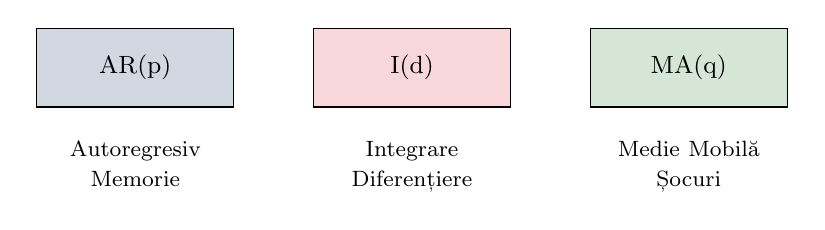
\begin{tikzpicture}[node distance=2cm, every node/.style={font=\small}]
            \node[draw, rectangle, fill=MainBlue!20, minimum width=2.5cm, minimum height=1cm] (AR) {AR(p)};
            \node[draw, rectangle, fill=Crimson!20, minimum width=2.5cm, minimum height=1cm, right=1cm of AR] (I) {I(d)};
            \node[draw, rectangle, fill=Forest!20, minimum width=2.5cm, minimum height=1cm, right=1cm of I] (MA) {MA(q)};

            \node[below=0.3cm of AR, text width=2.5cm, align=center] {\footnotesize Autoregresiv\\Memorie};
            \node[below=0.3cm of I, text width=2.5cm, align=center] {\footnotesize Integrare\\Diferențiere};
            \node[below=0.3cm of MA, text width=2.5cm, align=center] {\footnotesize Medie Mobilă\\Șocuri};
        \end{tikzpicture}
    \end{center}

    \vspace{0.2cm}

    {\small
    \begin{block}{Cazuri Speciale}
        \begin{itemize}\setlength{\itemsep}{0pt}
            \item ARIMA(p,0,q) = ARMA(p,q) $\succ$ staționar
            \item ARIMA(0,1,0) = Mers aleatoriu
            \item ARIMA(0,1,1) = IMA(1,1) $\succ$ netezire exponențială
            \item ARIMA(1,1,0) = ARI(1,1) $\succ$ AR(1) diferențiat
        \end{itemize}
    \end{block}
    }
    }
    \end{cminipage}
\end{frame}

\begin{frame}{Exemplu ARIMA(1,1,0)}
    \begin{cminipage}{0.95\textwidth}
    {\small
    \begin{exampleblock}{Model ARI(1,1)}
        \begin{itemize}\setlength{\itemsep}{0pt}
            \item $\Delta Y_t = c + \phi_1 \Delta Y_{t-1} + \varepsilon_t$
            \item Echivalent: $(1-\phi_1 L)(1-L)Y_t = c + \varepsilon_t$
        \end{itemize}
    \end{exampleblock}

    \vspace{0.1cm}

    \begin{block}{Interpretare}
        \begin{itemize}\setlength{\itemsep}{0pt}
            \item \textbf{Schimbările} în $Y_t$ urmează un proces AR(1)
            \item Dacă $|\phi_1| < 1$, schimbările sunt staționare
            \item $Y_t$ în sine are un trend stochastic
            \item Model comun pentru multe serii de timp economice
        \end{itemize}
    \end{block}
    }
    \end{cminipage}
\end{frame}

\begin{frame}{Exemplu ARIMA(0,1,1)}
    \begin{cminipage}{0.95\textwidth}
    {\small
    \begin{exampleblock}{Model IMA(1,1)}
        \begin{itemize}\setlength{\itemsep}{0pt}
            \item $\Delta Y_t = c + \varepsilon_t + \theta_1 \varepsilon_{t-1}$
            \item Echivalent: $(1-L)Y_t = c + (1+\theta_1 L)\varepsilon_t$
        \end{itemize}
    \end{exampleblock}

    \vspace{0.1cm}

    \begin{block}{Conexiunea cu Netezirea exponențială}
        \begin{itemize}\setlength{\itemsep}{0pt}
            \item Modelul IMA(1,1) este echivalent cu \textbf{netezirea exponențială simplă}:
                $$\hat{Y}_{t+1} = \alpha Y_t + (1-\alpha)\hat{Y}_t$$
            \item unde $\alpha = 1 + \theta_1$ (pentru $-1 < \theta_1 < 0$)
        \end{itemize}
    \end{block}
    }
    \end{cminipage}
\end{frame}

\begin{frame}{Rolul constantei în ARIMA}
    \begin{cminipage}{0.95\textwidth}
    {\small
    \begin{block}{Termenul Constant în ARIMA(p,d,q)}
        \begin{itemize}\setlength{\itemsep}{0pt}
            \item Când $d > 0$, constanta $c$ are o interpretare diferită:
            \item $\phi(L)(1-L)^d Y_t = c + \theta(L)\varepsilon_t$
        \end{itemize}
    \end{block}

    \vspace{0.1cm}

    \begin{alertblock}{Implicații Importante}
        \begin{itemize}\setlength{\itemsep}{0pt}
            \item Pentru $d=1$: $c$ reprezintă \textbf{drift-ul} (schimbarea medie): $\E[\Delta Y_t] = \frac{c}{1-\phi_1-\cdots-\phi_p}$
            \item Pentru $d=2$: $c$ afectează \textbf{curbura} trendului
            \item Adesea se presupune $c=0$ când $d \geq 1$
        \end{itemize}
    \end{alertblock}
    }
    \end{cminipage}
\end{frame}

%=============================================================================
% SECȚIUNEA 4: TESTE DE RĂDĂCINĂ UNITATE
%=============================================================================
\section{Teste de rădăcină unitate}

\begin{frame}{Portret de cercetător: Dickey \& Fuller}
    \vspace{-0.2cm}
    \begin{columns}[T]
        \begin{column}{0.22\textwidth}
            \centering
            \includegraphics[width=0.95\textwidth, height=0.22\textheight, keepaspectratio]{photo_david_dickey.jpg}
            \\[0.05cm]
            {\tiny\textcolor{MediumGray}{David Dickey (*1945)}}\\[0.02cm]
            \href{https://en.wikipedia.org/wiki/David_Dickey}{\faWikipediaW\ \textcolor{MainBlue}{\tiny Wikipedia (en)}}
        \end{column}
        \begin{column}{0.76\textwidth}
            \begin{block}{Biografie}
                {\footnotesize \begin{itemize}\setlength{\itemsep}{0pt}
                    \item \textbf{David Dickey}: statistician american la NC State University. Doctorand al lui Wayne Fuller la Iowa State
                    \item \textbf{Wayne Fuller}: statistician american, profesor la Iowa State University
                    \item Împreună au dezvoltat testul fundamental pentru rădăcini unitate în serii de timp
                \end{itemize}}
            \end{block}
        \end{column}
    \end{columns}
    \vspace{0.1cm}
    \begin{columns}[T]
        \begin{column}{0.22\textwidth}
            \centering
            \includegraphics[width=0.95\textwidth, height=0.22\textheight, keepaspectratio]{photo_wayne_fuller.jpg}
            \\[0.05cm]
            {\tiny\textcolor{MediumGray}{Wayne Fuller (1931--2022)}}\\[0.02cm]
            \href{https://en.wikipedia.org/wiki/Wayne_Fuller}{\faWikipediaW\ \textcolor{MainBlue}{\tiny Wikipedia (en)}}
        \end{column}
        \begin{column}{0.76\textwidth}
            \begin{exampleblock}{Contribuții principale}
                {\footnotesize \begin{itemize}\setlength{\itemsep}{0pt}
                    \item \textbf{Testul Dickey-Fuller} (1979) --- testul fundamental pentru rădăcini unitate
                    \item \textbf{Testul ADF} (Augmented Dickey-Fuller) --- extensie cu diferențe întârziate
                    \item \textbf{Tabele de valori critice} --- distribuții non-standard sub ipoteza nulă
                    \item Testarea riguroasă a ordinului de integrare pentru modelarea ARIMA
                \end{itemize}}
            \end{exampleblock}
        \end{column}
    \end{columns}
\end{frame}

\begin{frame}{Testarea pentru rădăcini unitate}
    \begin{cminipage}{0.95\textwidth}
    {\small
    \begin{block}{De ce Testăm?}
        \begin{itemize}\setlength{\itemsep}{0pt}
            \item \textbf{Scop}: înainte de a potrivi un model ARIMA, trebuie să determinăm:
            \begin{itemize}\setlength{\itemsep}{0pt}
                \item Este seria staționară? (Este $d=0$?)
                \item Dacă nu, câte diferențe sunt necesare? (Care este $d$?)
            \end{itemize}
        \end{itemize}
    \end{block}

    \vspace{0.1cm}

    \begin{block}{Teste comune de rădăcină unitate}
        \begin{itemize}\setlength{\itemsep}{0pt}
            \item \textbf{Dickey-Fuller (DF)} și \textbf{Augmented Dickey-Fuller (ADF)}
            \item \textbf{Phillips-Perron (PP)}
            \item \textbf{KPSS} (test de staționaritate $\succ$ ipoteză nulă inversată)
        \end{itemize}
    \end{block}
    }
    \end{cminipage}
\end{frame}

\begin{frame}{Testul Dickey-Fuller}
    \begin{cminipage}{0.95\textwidth}
    {\small
    \vspace{-0.2cm}
    {\small
    \begin{block}{Configurare}
        \begin{itemize}\setlength{\itemsep}{0pt}
            \item Considerăm modelul AR(1): $Y_t = \phi Y_{t-1} + \varepsilon_t$. Scădem $Y_{t-1}$:
            \item $\Delta Y_t = (\phi - 1)Y_{t-1} + \varepsilon_t = \gamma Y_{t-1} + \varepsilon_t$, unde $\gamma = \phi - 1$
        \end{itemize}
    \end{block}

    \vspace{0.05cm}

    \begin{block}{Ipoteze}
        \begin{itemize}\setlength{\itemsep}{0pt}
            \item $H_0$: $\gamma = 0$ (rădăcină unitate, $\phi = 1$, nestaționar)
            \item $H_1$: $\gamma < 0$ (staționar, $|\phi| < 1$)
        \end{itemize}
    \end{block}

    \vspace{0.05cm}

    \begin{alertblock}{Problemă Cheie}
        \begin{itemize}\setlength{\itemsep}{0pt}
            \item Sub $H_0$, statistica $t$ \textbf{nu} urmează o distribuție $t$ standard!
            \item Trebuie folosite valorile critice Dickey-Fuller
        \end{itemize}
    \end{alertblock}
    }
    }
    \end{cminipage}
\end{frame}

\begin{frame}{Variante ale testului Dickey-Fuller}
    \begin{cminipage}{0.95\textwidth}
    {\small
    \vspace{-0.2cm}
    {\small
    \begin{block}{Trei Specificări}
        \begin{enumerate}\setlength{\itemsep}{0pt}
            \item \textbf{Fără constantă, fără trend}: $\Delta Y_t = \gamma Y_{t-1} + \varepsilon_t$
            \item \textbf{Cu constantă (drift)}: $\Delta Y_t = \alpha + \gamma Y_{t-1} + \varepsilon_t$
            \item \textbf{Cu constantă și trend}: $\Delta Y_t = \alpha + \beta t + \gamma Y_{t-1} + \varepsilon_t$
        \end{enumerate}
    \end{block}

    \vspace{0.05cm}

    \begin{alertblock}{Alegerea Specificării Corecte}
        \begin{itemize}\setlength{\itemsep}{0pt}
            \item Examinați datele: au un trend vizibil?
            \item Includerea termenilor inutili reduce puterea
            \item Excluderea termenilor necesari duce la inferență incorectă
        \end{itemize}
    \end{alertblock}
    }
    }
    \end{cminipage}
\end{frame}

\begin{frame}{Testul Augmented Dickey-Fuller (ADF)}
    \begin{cminipage}{0.95\textwidth}
    {\small
    \vspace{-0.2cm}
    {\small
    \begin{block}{Problema cu DF Simplu}
        \begin{itemize}\setlength{\itemsep}{0pt}
            \item \textbf{Limitare}: dacă există dinamică AR dincolo de AR(1), reziduurile DF vor fi autocorelate
        \end{itemize}
    \end{block}

    \vspace{0.1cm}

    \begin{defn}[Testul ADF]
        \begin{itemize}\setlength{\itemsep}{0pt}
            \item \textbf{Ecuație}: $\Delta Y_t = \alpha + \beta t + \gamma Y_{t-1} + \sum_{j=1}^{k} \delta_j \Delta Y_{t-j} + \varepsilon_t$
            \item \textbf{Test}: $H_0: \gamma = 0$ folosind valorile critice ADF
        \end{itemize}
    \end{defn}

    \vspace{0.1cm}

    \begin{block}{Alegerea Lungimii Lag-ului $k$}
        \begin{itemize}
            \item Folosiți criterii informaționale (AIC, BIC)
            \item Începeți cu $k_{max}$, reduceți până ultimul lag este semnificativ
        \end{itemize}
    \end{block}
    }
    }
    \end{cminipage}
\end{frame}

\begin{frame}{Testul ADF: ilustrație vizuală}
    \begin{center}
        \includegraphics[width=0.95\textwidth, height=0.78\textheight, keepaspectratio]{ch3_def_adf.pdf}
    \end{center}
    \quantlet{TSA\_ch3\_def\_adf}{https://github.com/QuantLet/TSA/tree/main/TSA_ch3/TSA_ch3_def_adf}
\end{frame}

\begin{frame}{Testul ADF: ilustrație vizuală}
    \vspace{-0.2cm}
    {\footnotesize
    \begin{block}{Observație}
        \begin{itemize}\setlength{\itemsep}{0pt}
            \item \textbf{Stânga}: serie staționară $\succ$ ADF respinge rădăcina unitate
            \item \textbf{Dreapta}: nestaționară $\succ$ ADF nu respinge
        \end{itemize}
    \end{block}
    }
\end{frame}

\begin{frame}{Valori critice ADF}
    \begin{cminipage}{0.95\textwidth}
    {\small
    \vspace{-0.2cm}
    {\small
    \begin{table}
        \centering
        \begin{tabular}{lccc}
            \toprule
            \textbf{Model} & \textbf{1\%} & \textbf{5\%} & \textbf{10\%} \\
            \midrule
            Fără constantă, fără trend & $-2.58$ & $-1.95$ & $-1.62$ \\
            Cu constantă & $-3.43$ & $-2.86$ & $-2.57$ \\
            Cu constantă și trend & $-3.96$ & $-3.41$ & $-3.13$ \\
            \bottomrule
        \end{tabular}
    \end{table}
    }
    \vspace{-0.1cm}
    \begin{block}{Regula de Decizie}
        {\small
        \begin{itemize}
            \item Statistică de test $<$ valoare critică $\succ$ Respingem $H_0$ (staționar)
            \item Statistică de test $\geq$ valoare critică $\succ$ Nu respingem (rădăcină unitate)
        \end{itemize}
        }
    \end{block}
    }
    \end{cminipage}
\end{frame}

\begin{frame}{Testul Phillips-Perron (PP)}
    \begin{cminipage}{0.95\textwidth}
    {\small
    \vspace{-0.15cm}
    {\small
    \begin{block}{Motivație}
        \begin{itemize}\setlength{\itemsep}{0pt}
            \item \textbf{Ipoteze}: $H_0$: Rădăcină unitate vs $H_1$: Staționar (ca ADF)
            \item \textbf{Diferență}: folosește o corecție non-parametrică pentru corelația serială
            \begin{itemize}
                \item Nu adaugă diferențe întârziate ca ADF
            \end{itemize}
        \end{itemize}
    \end{block}

    \begin{block}{Statistică de Test}
        \begin{itemize}\setlength{\itemsep}{0pt}
            \item \textbf{Formula}: $Z_t = t_{\hat{\gamma}} \cdot \sqrt{\frac{\hat{\sigma}^2}{\hat{\lambda}^2}} - \frac{T(\hat{\lambda}^2 - \hat{\sigma}^2)(se(\hat{\gamma}))}{2\hat{\lambda}^2 \cdot s}$
            \item \textbf{Notație}: $\hat{\lambda}^2$ este estimarea consistentă a varianței pe termen lung (Newey-West)
        \end{itemize}
    \end{block}

    \begin{exampleblock}{Avantaje față de ADF}
        \begin{itemize}\setlength{\itemsep}{0pt}
            \item Robust la heteroscedasticitate și corelație serială
            \item Nu necesită selectarea lungimii lag-ului (folosește lățime de bandă)
        \end{itemize}
    \end{exampleblock}
    }
    }
    \end{cminipage}
\end{frame}

\begin{frame}{Testul KPSS}
    \begin{cminipage}{0.95\textwidth}
    {\small
    \vspace{-0.2cm}
    {\small
    \begin{block}{Ipoteze Inversate}
        \begin{itemize}\setlength{\itemsep}{0pt}
            \item \textbf{Spre deosebire de ADF}: $H_0$: Staționar vs $H_1$: Rădăcină unitate
            \begin{itemize}
                \item Ipoteza nulă este inversată față de ADF/PP
            \end{itemize}
        \end{itemize}
    \end{block}

    \vspace{0.1cm}

    \begin{block}{Procedura KPSS}
        \begin{itemize}\setlength{\itemsep}{0pt}
            \item \textbf{Descompunere}: $Y_t = \xi t + r_t + \varepsilon_t$ unde $r_t = r_{t-1} + u_t$
            \item \textbf{Test}: verificăm dacă $\Var(u_t) = 0$
            \begin{itemize}
                \item Dacă da, componenta aleatoare $r_t$ este constantă
            \end{itemize}
        \end{itemize}
    \end{block}

    \vspace{0.1cm}

    \begin{exampleblock}{Utilizare Complementară cu ADF}
        \begin{itemize}
            \item ADF respinge, KPSS nu respinge $\succ$ Staționar
            \item ADF nu respinge, KPSS respinge $\succ$ Rădăcină unitate
            \item Ambele resping sau niciunul $\succ$ Neconcludent
        \end{itemize}
    \end{exampleblock}
    }
    }
    \end{cminipage}
\end{frame}

%=============================================================================
% SECȚIUNEA 5: IDENTIFICAREA MODELULUI
%=============================================================================
\section{Identificarea modelului ARIMA}

\begin{frame}{Metodologia Box-Jenkins}
    \begin{cminipage}{0.95\textwidth}
    \begin{center}
        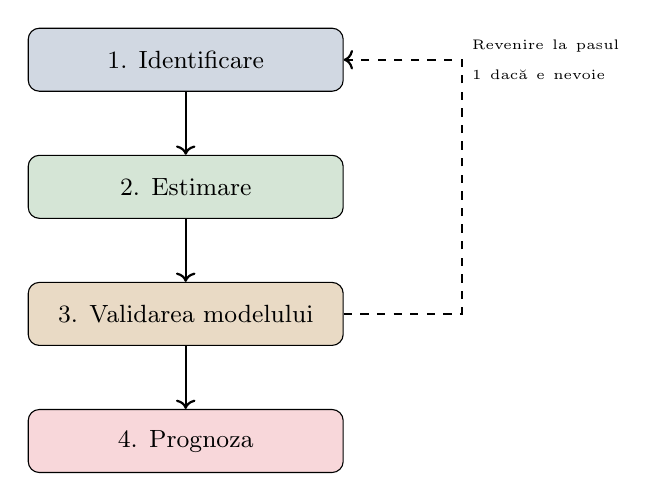
\begin{tikzpicture}[node distance=1.5cm, every node/.style={font=\small}]
            \node[draw, rectangle, rounded corners, fill=MainBlue!20, minimum width=4cm, minimum height=0.8cm] (id) {1. Identificare};
            \node[draw, rectangle, rounded corners, fill=Forest!20, minimum width=4cm, minimum height=0.8cm, below=0.8cm of id] (est) {2. Estimare};
            \node[draw, rectangle, rounded corners, fill=Amber!30, minimum width=4cm, minimum height=0.8cm, below=0.8cm of est] (diag) {3. Validarea modelului};
            \node[draw, rectangle, rounded corners, fill=Crimson!20, minimum width=4cm, minimum height=0.8cm, below=0.8cm of diag] (fore) {4. Prognoza};

            \draw[->, thick] (id) -- (est);
            \draw[->, thick] (est) -- (diag);
            \draw[->, thick] (diag) -- (fore);
            \draw[->, thick, dashed] (diag.east) -- ++(1.5,0) |- (id.east) node[midway, right, text width=2cm] {\tiny Revenire la pasul 1 dacă e nevoie};
        \end{tikzpicture}
    \end{center}
    \end{cminipage}
\end{frame}

\begin{frame}{Pasul 1: Determinarea lui $d$}
    \begin{cminipage}{0.95\textwidth}
    {\small
    \begin{block}{Procedură}
        \begin{enumerate}\setlength{\itemsep}{0pt}
            \item Reprezentați grafic seria de timp $\succ$ căutați trenduri, varianță în schimbare
            \item Examinați ACF $\succ$ descreștere lentă sugerează nestaționaritate
            \item Aplicați teste de rădăcină unitate (ADF, KPSS)
            \item Dacă nestaționară, diferențiați și repetăți
        \end{enumerate}
    \end{block}

    \vspace{0.1cm}

    \begin{exampleblock}{Ghiduri Practice}
        \begin{itemize}\setlength{\itemsep}{0pt}
            \item Majoritatea seriilor economice: $d = 1$ este suficient
            \item Rar avem nevoie de $d > 2$
            \item Dacă ACF al $\Delta Y_t$ tot scade lent, încercați $d = 2$
            \item Atenție la supra-diferențiere (ACF cu $\rho_1 \approx -0.5$)
        \end{itemize}
    \end{exampleblock}
    }
    \end{cminipage}
\end{frame}

\begin{frame}{Pasul 2: Determinarea lui $p$ și $q$}
    \begin{cminipage}{0.95\textwidth}
    {\small
    \vspace{-0.3cm}
    {\small
    \begin{block}{După Diferențiere}
        \begin{itemize}\setlength{\itemsep}{0pt}
            \item \textbf{Principiu}: odată ce $W_t = \Delta^d Y_t$ este staționar, folosiți ACF/PACF pentru a identifica ARMA($p$,$q$)
        \end{itemize}
    \end{block}

    \vspace{-0.05cm}

    \begin{center}
        \begin{tabular}{lcc}
            \toprule
            \textbf{Model} & \textbf{ACF} & \textbf{PACF} \\
            \midrule
            AR($p$) & Scade exponențial & Se anulează după lag $p$ \\
            MA($q$) & Se anulează după lag $q$ & Scade exponențial \\
            ARMA($p$,$q$) & Scade & Scade \\
            \bottomrule
        \end{tabular}
    \end{center}

    \vspace{-0.05cm}

    \begin{block}{Criterii informaționale}
        \begin{itemize}\setlength{\itemsep}{0pt}
            \item \textbf{Când}: tiparele ACF/PACF sunt neclare
            \item \textbf{AIC}: $-2\ln(L) + 2k$; \quad \textbf{BIC}: $-2\ln(L) + k\ln(n)$
                  {\scriptsize ($L$ = verosimilitate, $k$ = parametri, $n$ = eșantion)}
            \item Mai mic este mai bun; BIC penalizează complexitatea mai mult
        \end{itemize}
    \end{block}
    }
    }
    \end{cminipage}
\end{frame}

\begin{frame}{Algoritmi Auto-ARIMA}
    \begin{cminipage}{0.95\textwidth}
    {\small
    \vspace{-0.15cm}
    {\small
    \begin{block}{Selecție automată a modelului}
        \begin{itemize}\setlength{\itemsep}{0pt}
            \item Software-ul modern poate selecta automat $(p,d,q)$:
            \begin{itemize}\setlength{\itemsep}{0pt}
                \item Python: \texttt{pmdarima.auto\_arima()} \quad R: \texttt{forecast::auto.arima()}
            \end{itemize}
        \end{itemize}
    \end{block}

    \begin{block}{Cum funcționează Auto-ARIMA}
        \begin{enumerate}\setlength{\itemsep}{0pt}
            \item Folosește teste de rădăcină unitate pentru a determina $d$
            \item Potrivește modele pentru diverse combinații $(p,q)$
            \item Selectează modelul cu cel mai mic AIC/BIC
            \item Opțional folosește căutare pas cu pas pentru eficiență
        \end{enumerate}
    \end{block}

    \vspace{0.1cm}
    \textcolor{IDAred}{\textbf{Atenție:}} Selecția automată este utilă dar nu garantată --- verificați întotdeauna validitatea modelului!
    }
    }
    \end{cminipage}
\end{frame}

%=============================================================================
% SECȚIUNEA 6: ESTIMARE
%=============================================================================
\section{Estimarea ARIMA}

\begin{frame}{Metode de estimare}
    \begin{cminipage}{0.95\textwidth}
    {\small
    \begin{block}{Estimarea prin metoda verosimilității maxime (MLE)}
        \begin{itemize}\setlength{\itemsep}{0pt}
            \item Abordarea standard pentru ARIMA:
            \begin{itemize}\setlength{\itemsep}{0pt}
                \item Presupune $\varepsilon_t \sim N(0, \sigma^2)$
                \item Maximizează funcția de verosimilitate
                \item Oferă estimatori consistenți, eficienți
                \item Furnizează erori standard pentru inferență
            \end{itemize}
        \end{itemize}
    \end{block}

    \vspace{0.1cm}

    \begin{block}{MLE Condiționată vs Exactă}
        \begin{itemize}\setlength{\itemsep}{0pt}
            \item \textbf{MLE Condiționată}: Condiționează pe valorile inițiale
            \item \textbf{MLE Exactă}: Tratează valorile inițiale ca necunoscute
            \item Diferența diminuează pe măsură ce dimensiunea eșantionului crește
        \end{itemize}
    \end{block}
    }
    \end{cminipage}
\end{frame}

\begin{frame}{Log-verosimilitatea condiționată}
    \begin{cminipage}{0.95\textwidth}
    {\small
    \vspace{-0.2cm}
    {\footnotesize
    \begin{block}{Funcția de log-verosimilitate gaussiană}
        \begin{itemize}\setlength{\itemsep}{0pt}
            \item $\ell(\boldsymbol{\theta}, \sigma^2) = -\frac{T}{2}\ln(2\pi) - \frac{T}{2}\ln(\sigma^2) - \frac{1}{2\sigma^2}\sum_{t=1}^{T} e_t^2(\boldsymbol{\theta})$
            \item $e_t(\boldsymbol{\theta}) = X_t - \hat{X}_{t|t-1}$ sunt \textbf{erorile de predicție la un pas}
            \item $\boldsymbol{\theta} = (\phi_1, \ldots, \phi_p, \theta_1, \ldots, \theta_q, c)$
        \end{itemize}
    \end{block}

    \begin{exampleblock}{Exemplu: ARIMA(1,1,1)}
        \begin{itemize}\setlength{\itemsep}{0pt}
            \item Erorile de predicție: $e_t = \Delta X_t - \phi_1 \Delta X_{t-1} - \theta_1 e_{t-1} - c$
            \item MLE condiționată: fixează $e_0 = 0$, calculează $e_1, \ldots, e_T$, maximizează $\ell$
        \end{itemize}
    \end{exampleblock}

    \begin{alertblock}{Estimarea lui $\sigma^2$}
        \begin{itemize}\setlength{\itemsep}{0pt}
            \item La parametrii optimi $\hat{\boldsymbol{\theta}}$: $\hat{\sigma}^2 = \frac{1}{T}\sum_{t=1}^{T} e_t^2(\hat{\boldsymbol{\theta}})$
        \end{itemize}
    \end{alertblock}
    }
    }
    \end{cminipage}
\end{frame}

\begin{frame}{Restricții asupra parametrilor}
    \begin{cminipage}{0.95\textwidth}
    {\small
    \begin{alertblock}{Staționaritate și invertibilitate}
        \begin{itemize}\setlength{\itemsep}{0pt}
            \item Modelul ARIMA estimat ar trebui să satisfacă:
            \begin{itemize}\setlength{\itemsep}{0pt}
                \item \textbf{Staționaritate AR}: Rădăcinile lui $\phi(z) = 0$ în afara cercului unitate
                \item \textbf{Invertibilitate MA}: Rădăcinile lui $\theta(z) = 0$ în afara cercului unitate
            \end{itemize}
        \end{itemize}
    \end{alertblock}

    \vspace{0.1cm}

    \begin{block}{Verificare în Practică}
        \begin{itemize}\setlength{\itemsep}{0pt}
            \item Majoritatea software-ului raportează:
            \begin{itemize}\setlength{\itemsep}{0pt}
                \item Coeficienți estimați cu erori standard
                \item Rădăcinile polinoamelor AR și MA
                \item Avertisment dacă este detectată aproape-rădăcină-unitate
            \end{itemize}
        \end{itemize}
    \end{block}
    }
    \end{cminipage}
\end{frame}

%=============================================================================
% SECȚIUNEA 7: DIAGNOSTICARE
%=============================================================================
\section{Diagnosticul modelului}

\begin{frame}{Diagnosticul modelului ARIMA}
    \begin{cminipage}{0.95\textwidth}
    {\small
    \begin{block}{Verificări esențiale (aceleași ca pentru ARMA, cf.\ Cap.\ 2)}
        \begin{itemize}\setlength{\itemsep}{0pt}
            \item Dacă modelul este corect, reziduurile $\hat{\varepsilon}_t$ trebuie să fie zgomot alb:
            \begin{enumerate}\setlength{\itemsep}{0pt}
                \item \textbf{ACF/PACF rezidual}: fără vârfuri semnificative
                \item \textbf{Testul Ljung-Box}: p-value $> 0.05$ $\succ$ fără autocorelare
                \item \textbf{Graficul Q-Q}: verificarea normalității
                \item \textbf{Heteroscedasticitate}: varianță constantă a reziduurilor
            \end{enumerate}
        \end{itemize}
    \end{block}

    \vspace{0.1cm}

    \begin{alertblock}{Aspecte specifice ARIMA}
        \begin{itemize}\setlength{\itemsep}{0pt}
            \item Testul Ljung-Box: alegeți $m \approx \ln(n)$ sau $m = 10$ (trimestrial), $m = 20$ (lunar)
            \item Grade de libertate: $\chi^2(m-p-q)$, ajustate pentru $p$ și $q$ estimați
            \item Dacă testul eșuează: adăugați termeni AR/MA sau verificați rupturi structurale
        \end{itemize}
    \end{alertblock}
    }
    \end{cminipage}
\end{frame}

\begin{frame}{Testul Ljung-Box}
    \begin{cminipage}{0.95\textwidth}
    {\small
    \begin{defn}[Statistica Q Ljung-Box]
        $Q(m) = n(n+2) \sum_{k=1}^{m} \frac{\hat{\rho}_k^2}{n-k}$. Sub $H_0$ (fără autocorelare): $Q(m) \sim \chi^2(m-p-q)$
    \end{defn}

    \vspace{0.1cm}

    \begin{block}{Utilizare}
        \begin{itemize}\setlength{\itemsep}{0pt}
            \item Alegeți $m \approx \ln(n)$ sau $m = 10$ trimestrial, $m = 20$ lunar
            \item Gradele de libertate se ajustează pentru parametrii estimați
            \item Respingeți dacă $Q(m)$ depășește valoarea critică
        \end{itemize}
    \end{block}

    \vspace{0.1cm}

    \begin{alertblock}{Dacă testul eșuează}
        Luați în considerare adăugarea de termeni AR sau MA, sau verificați rupturile structurale.
    \end{alertblock}
    }
    \end{cminipage}
\end{frame}

%=============================================================================
% SECȚIUNEA 8: PROGNOZA
%=============================================================================
\section{Prognoza cu ARIMA}

\begin{frame}{Prognoze punctuale}
    \begin{cminipage}{0.95\textwidth}
    {\small
    \begin{block}{Prognoza cu MSE Minim}
        \begin{itemize}\setlength{\itemsep}{0pt}
            \item Prognoză optimă la $h$ pași: $\hat{Y}_{T+h|T} = \E[Y_{T+h} | Y_T, Y_{T-1}, \ldots]$
        \end{itemize}
    \end{block}

    \vspace{0.1cm}

    \begin{exampleblock}{Prognoza ARIMA(1,1,1)}
        \begin{itemize}\setlength{\itemsep}{0pt}
            \item \textbf{Model}: $(1-\phi_1 L)(1-L)Y_t = c + (1+\theta_1 L)\varepsilon_t$
            \item \textbf{Un pas}: $\hat{Y}_{T+1|T} = c + Y_T + \phi_1(Y_T - Y_{T-1}) + \theta_1 \hat{\varepsilon}_T$
            \item \textbf{Multi-pas}: înlocuiți $\varepsilon_{T+j}$ cu 0, $Y_{T+j}$ cu $\hat{Y}_{T+j|T}$
        \end{itemize}
    \end{exampleblock}
    }
    \end{cminipage}
\end{frame}

\begin{frame}{Intervale de prognoză}
    \begin{cminipage}{0.95\textwidth}
    {\small
    \begin{block}{Incertitudinea prognozei}
        \begin{itemize}\setlength{\itemsep}{0pt}
            \item Varianța erorii la $h$ pași: $\Var(e_{T+h}) = \sigma^2 \sum_{j=0}^{h-1} \psi_j^2$, unde $\psi_j$ sunt coeficienții MA($\infty$)
        \end{itemize}
    \end{block}

    \vspace{0.1cm}

    \begin{block}{Intervale de încredere}
        \begin{itemize}\setlength{\itemsep}{0pt}
            \item Sub normalitate, interval $(1-\alpha)$\%: $\hat{Y}_{T+h|T} \pm z_{\alpha/2} \sqrt{\Var(e_{T+h})}$
        \end{itemize}
    \end{block}

    \vspace{0.1cm}

    \begin{alertblock}{Proprietate Cheie pentru Serii I(1)}
        \begin{itemize}\setlength{\itemsep}{0pt}
            \item Pentru procese integrate, varianța prognozei crește nelimitat când $h \to \infty$
            \item Intervalele se lărgesc în timp!
        \end{itemize}
    \end{alertblock}
    }
    \end{cminipage}
\end{frame}

\begin{frame}{Prognoze pe termen lung pentru ARIMA}
    \begin{cminipage}{0.95\textwidth}
    {\small
    \begin{block}{Comportament când $h \to \infty$}
        \begin{itemize}\setlength{\itemsep}{0pt}
            \item \textbf{Cu drift $c$}: Prognoze punctuale $\succ$ trend liniar; IC $\succ$ lățimea crește cu $\sqrt{h}$
            \item \textbf{Fără drift}: Prognoze punctuale $\succ$ converg la ultima valoare observată; IC $\succ$ tot cresc nelimitat
        \end{itemize}
    \end{block}

    \vspace{0.1cm}

    \begin{alertblock}{Implicație Practică}
        \begin{itemize}\setlength{\itemsep}{0pt}
            \item Prognozele ARIMA sunt cele mai fiabile pentru orizonturi scurte
            \item Prognozele pe termen lung au benzi de incertitudine foarte largi
        \end{itemize}
    \end{alertblock}
    }
    \end{cminipage}
\end{frame}

\begin{frame}{Prognoza rolling: concept}
    \begin{cminipage}{0.95\textwidth}
    {\small
    \vspace{-0.2cm}
    {\small
    \begin{block}{Ce este Prognoza Rolling?}
        \begin{itemize}\setlength{\itemsep}{0pt}
            \item Tehnică pentru evaluarea acurateții prognozei în afara eșantionului:
            \begin{enumerate}\setlength{\itemsep}{0pt}
                \item Fixăm o \textbf{fereastră de antrenament} de dimensiune $w$
                \item Estimăm modelul pe observațiile $t = 1, \ldots, w$
                \item Prognozăm $h$ pași înainte: $\hat{Y}_{w+h|w}$
                \item \textbf{Deplasăm} fereastra înainte cu o perioadă
                \item Repetăm până la sfârșitul eșantionului
            \end{enumerate}
        \end{itemize}
    \end{block}

    \vspace{0.05cm}

    \begin{exampleblock}{De ce Prognoze Rolling?}
        \begin{itemize}\setlength{\itemsep}{0pt}
            \item Mimează scenariul de prognoză în timp real
            \item Oferă multiple erori de prognoză pentru evaluare
            \item Evită supraajustarea pe întregul eșantion
        \end{itemize}
    \end{exampleblock}
    }
    }
    \end{cminipage}
\end{frame}

\begin{frame}{Fereastră fixă vs expandabilă}
    \begin{center}
    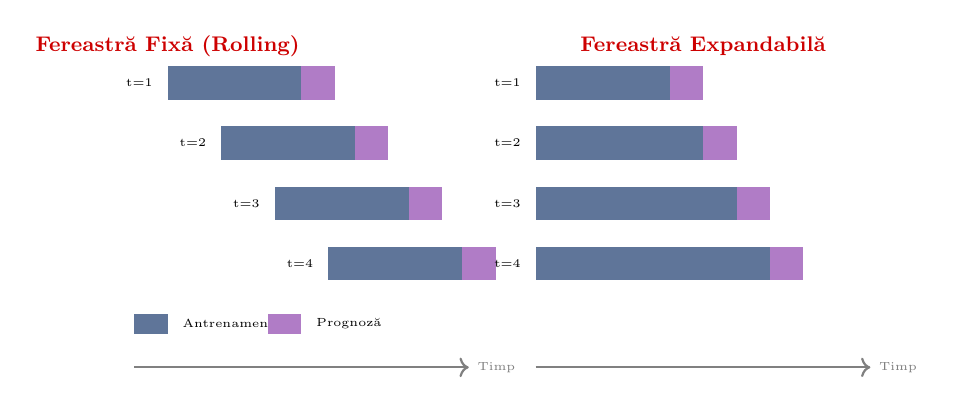
\begin{tikzpicture}[scale=0.85, transform shape]
        % Title for Fixed Window
        \node[font=\bfseries\small, color=IDAred] at (0, 3.8) {Fereastră Fixă (Rolling)};

        % Fixed window iterations
        \foreach \i in {0,1,2,3} {
            \pgfmathsetmacro{\y}{3 - \i*0.9}
            \fill[MainBlue!70] ({\i*0.8}, \y) rectangle ({2+\i*0.8}, {\y+0.5});
            \fill[Purple!70] ({2+\i*0.8}, \y) rectangle ({2.5+\i*0.8}, {\y+0.5});
            \node[font=\tiny, left] at ({\i*0.8-0.1}, {\y+0.25}) {t=\pgfmathparse{int(\i+1)}\pgfmathresult};
        }
        \fill[MainBlue!70] (-0.5, -0.5) rectangle (0, -0.2);
        \node[font=\tiny, right] at (0.1, -0.35) {Antrenament};
        \fill[Purple!70] (1.5, -0.5) rectangle (2, -0.2);
        \node[font=\tiny, right] at (2.1, -0.35) {Prognoză};

        % Title for Expanding Window
        \node[font=\bfseries\small, color=IDAred] at (8, 3.8) {Fereastră Expandabilă};

        % Expanding window iterations
        \foreach \i in {0,1,2,3} {
            \pgfmathsetmacro{\y}{3 - \i*0.9}
            \fill[MainBlue!70] (5.5, \y) rectangle ({7.5+\i*0.5}, {\y+0.5});
            \fill[Purple!70] ({7.5+\i*0.5}, \y) rectangle ({8+\i*0.5}, {\y+0.5});
            \node[font=\tiny, left] at (5.4, {\y+0.25}) {t=\pgfmathparse{int(\i+1)}\pgfmathresult};
        }

        \draw[->, thick, color=MediumGray] (-0.5, -1) -- (4.5, -1) node[right, font=\tiny] {Timp};
        \draw[->, thick, color=MediumGray] (5.5, -1) -- (10.5, -1) node[right, font=\tiny] {Timp};
    \end{tikzpicture}
    \end{center}
    \vspace{-0.2cm}
    \begin{block}{Comparație}
        \begin{itemize}\setlength{\itemsep}{0pt}
            \item \textbf{Fixă}: Fereastra alunecă înainte, dimensiune constantă --- se adaptează la schimbări de regim
            \item \textbf{Expandabilă}: Fereastra crește în timp --- folosește toate datele istorice
        \end{itemize}
    \end{block}
\end{frame}

\begin{frame}{Prognoză 1-pas vs multi-pas}
    \begin{columns}[T]
        \begin{column}{0.48\textwidth}
            \begin{block}{1-Pas Înainte (Recursiv)}
                \begin{itemize}\setlength{\itemsep}{1pt}
                    \item Prognozează doar perioada următoare
                    \begin{itemize}
                        \item Re-estimează modelul după fiecare pas
                        \item Folosește valoarea reală odată observată
                    \end{itemize}
                    \item Cea mai precisă pentru orizonturi scurte
                \end{itemize}
            \end{block}
        \end{column}
        \begin{column}{0.48\textwidth}
            \begin{block}{Multi-Pas (Direct)}
                \begin{itemize}\setlength{\itemsep}{1pt}
                    \item Prognozează mai multe perioade înainte
                    \begin{itemize}
                        \item Fără re-estimare între pași
                        \item Folosește valori prognozate ca input
                    \end{itemize}
                    \item Incertitudinea se acumulează cu orizontul
                \end{itemize}
            \end{block}
        \end{column}
    \end{columns}
    \vspace{0.3cm}
    \begin{center}
    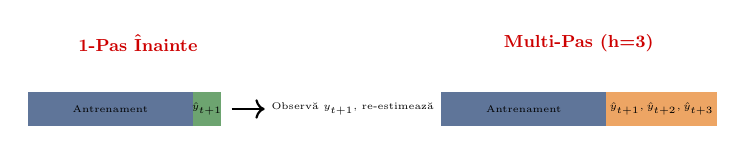
\begin{tikzpicture}[scale=0.7, transform shape]
        \node[font=\small\bfseries, color=IDAred] at (0, 1.5) {1-Pas Înainte};
        \fill[MainBlue!70] (-2, 0) rectangle (1, 0.6);
        \fill[Forest!70] (1, 0) rectangle (1.5, 0.6);
        \node[font=\tiny] at (-0.5, 0.3) {Antrenament};
        \node[font=\tiny] at (1.25, 0.3) {$\hat{y}_{t+1}$};
        \draw[->, thick] (1.7, 0.3) -- (2.3, 0.3);
        \node[font=\tiny, right] at (2.3, 0.3) {Observă $y_{t+1}$, re-estimează};

        \node[font=\small\bfseries, color=IDAred] at (8, 1.5) {Multi-Pas (h=3)};
        \fill[MainBlue!70] (5.5, 0) rectangle (8.5, 0.6);
        \fill[Orange!70] (8.5, 0) rectangle (10.5, 0.6);
        \node[font=\tiny] at (7, 0.3) {Antrenament};
        \node[font=\tiny] at (9.5, 0.3) {$\hat{y}_{t+1}, \hat{y}_{t+2}, \hat{y}_{t+3}$};
    \end{tikzpicture}
    \end{center}
\end{frame}

\begin{frame}{Prognoza rolling: exemplu pas cu pas}
    \begin{cminipage}{0.95\textwidth}
    {\small
    \vspace{-0.3cm}
    {\footnotesize
    \begin{exampleblock}{Configurare: ARIMA(1,1,0) cu $\phi_1 = 0.6$}
        \begin{itemize}\setlength{\itemsep}{0pt}
            \item Model: $\Delta Y_t = \phi_1 \Delta Y_{t-1} + \varepsilon_t$ unde $\Delta Y_t = Y_t - Y_{t-1}$
        \end{itemize}
    \end{exampleblock}

    \vspace{0.05cm}

    \begin{block}{Date la Momentul $T$}
        \begin{itemize}\setlength{\itemsep}{0pt}
            \item $Y_{T-2} = 100$, $Y_{T-1} = 103$, $Y_T = 108$ $\succ$ $\Delta Y_{T-1} = 3$, $\Delta Y_T = 5$
        \end{itemize}
    \end{block}

    \vspace{0.05cm}

    \begin{alertblock}{Prognoza Punctuală la 1 Pas}
        \vspace{-0.3cm}
        \begin{align*}
            \hat{\Delta Y}_{T+1|T} &= \phi_1 \cdot \Delta Y_T = 0.6 \times 5 = 3 \\[-0.2cm]
            \hat{Y}_{T+1|T} &= Y_T + \hat{\Delta Y}_{T+1|T} = 108 + 3 = \boxed{111}
        \end{align*}
        \vspace{-0.3cm}
    \end{alertblock}
    }
    }
    \end{cminipage}
\end{frame}

\begin{frame}{Prognoze punctuale multi-pas}
    \begin{cminipage}{0.95\textwidth}
    {\small
    \vspace{-0.2cm}
    {\footnotesize
    \begin{block}{Prognoza la 2 Pași}
        \vspace{-0.3cm}
        \begin{align*}
            \hat{\Delta Y}_{T+2|T} &= \phi_1 \cdot \hat{\Delta Y}_{T+1|T} = 0.6 \times 3 = 1.8 \\[-0.2cm]
            \hat{Y}_{T+2|T} &= \hat{Y}_{T+1|T} + \hat{\Delta Y}_{T+2|T} = 111 + 1.8 = \boxed{112.8}
        \end{align*}
        \vspace{-0.3cm}
    \end{block}

    \vspace{0.05cm}

    \begin{block}{Formula Generală pentru Prognoza la $h$ Pași (ARIMA(1,1,0))}
        \vspace{-0.3cm}
        \begin{align*}
            \hat{\Delta Y}_{T+h|T} &= \phi_1^h \cdot \Delta Y_T \\[-0.2cm]
            \hat{Y}_{T+h|T} &= Y_T + \Delta Y_T \cdot \frac{\phi_1(1-\phi_1^h)}{1-\phi_1}
        \end{align*}
        \vspace{-0.3cm}
    \end{block}

    \vspace{0.05cm}

    \begin{exampleblock}{Numeric: Prognoza la 3 Pași}
        \vspace{-0.1cm}
        $\hat{Y}_{T+3|T} = 108 + 5 \times \frac{0.6(1-0.6^3)}{1-0.6} = 108 + 5 \times 1.176 = \boxed{113.88}$
        \vspace{-0.1cm}
    \end{exampleblock}
    }
    }
    \end{cminipage}
\end{frame}

\begin{frame}{Intervale de încredere: formule}
    \begin{cminipage}{0.95\textwidth}
    {\small
    \begin{block}{Varianța erorii de prognoză}
        \begin{itemize}\setlength{\itemsep}{0pt}
            \item Pentru ARIMA(1,1,0) la $h$ pași: $\Var(e_{T+h|T}) = \sigma^2 \left(1 + \sum_{j=1}^{h-1} \psi_j^2 \right)$
            \item $\psi_j = 1 + \phi_1 + \cdots + \phi_1^{j} = \frac{1-\phi_1^{j+1}}{1-\phi_1}$ pentru $j \geq 0$
        \end{itemize}
    \end{block}

    \vspace{0.1cm}

    \begin{alertblock}{Interval de Încredere $(1-\alpha)$\%}
        \begin{itemize}\setlength{\itemsep}{0pt}
            \item $\hat{Y}_{T+h|T} \pm z_{\alpha/2} \cdot \sqrt{\Var(e_{T+h|T})}$
            \item Pentru IC 95\%: $z_{0.025} = 1.96$
        \end{itemize}
    \end{alertblock}
    }
    \end{cminipage}
\end{frame}

\begin{frame}{Interval de încredere: exemplu numeric}
    \begin{cminipage}{0.95\textwidth}
    {\small
    \vspace{-0.2cm}
    {\footnotesize
    \begin{exampleblock}{Date: $\sigma^2 = 4$, $\phi_1 = 0.6$, $\hat{Y}_{T+1|T} = 111$}
    \end{exampleblock}

    \vspace{0.05cm}

    \begin{block}{IC la 1 Pas}
        \vspace{-0.3cm}
        \begin{align*}
            \Var(e_{T+1|T}) &= \sigma^2 = 4 \\[-0.2cm]
            \text{IC 95\%} &= 111 \pm 1.96 \times \sqrt{4} = 111 \pm 3.92 = \boxed{[107.08, \; 114.92]}
        \end{align*}
        \vspace{-0.3cm}
    \end{block}

    \vspace{0.05cm}

    \begin{block}{IC la 2 Pași (pentru $\hat{Y}_{T+2|T} = 112.8$)}
        \vspace{-0.3cm}
        \begin{align*}
            \psi_1 &= 1 + \phi_1 = 1.6, \quad \Var(e_{T+2|T}) = 4(1 + 1.6^2) = 14.24 \\[-0.2cm]
            \text{IC 95\%} &= 112.8 \pm 1.96 \times \sqrt{14.24} = 112.8 \pm 7.40 = \boxed{[105.40, \; 120.20]}
        \end{align*}
        \vspace{-0.3cm}
    \end{block}

    \begin{alertblock}{Notă}
        \begin{itemize}\setlength{\itemsep}{0pt}
            \item IC se lărgește pe măsură ce orizontul de predicție crește!
        \end{itemize}
    \end{alertblock}
    }
    }
    \end{cminipage}
\end{frame}

\begin{frame}{Ilustrație fereastră rolling}
    \begin{center}
        \includegraphics[width=0.95\textwidth, height=0.78\textheight, keepaspectratio]{ch3_rolling_forecast.pdf}
    \end{center}
    \quantlet{TSA\_ch3\_rolling\_forecast}{https://github.com/QuantLet/TSA/tree/main/TSA_ch3/TSA_ch3_rolling_forecast}
\end{frame}

\begin{frame}{Ilustrație fereastră rolling}
    \vspace{-0.2cm}
    {\footnotesize
    \begin{exampleblock}{}
        \begin{itemize}\setlength{\itemsep}{0pt}
            \item Fiecare fereastră produce o prognoză la 1 pas
            \item Comparăm prognozele cu valorile reale pentru a calcula RMSE, MAE
            \item Fereastra rolling menține estimarea modelului actualizată
        \end{itemize}
    \end{exampleblock}
    }
\end{frame}

\begin{frame}[fragile]{Prognoza Rolling: Cod Python}
    \begin{cminipage}{0.95\textwidth}
    \vspace{-0.3cm}
    {\scriptsize
    \begin{block}{Implementare}
        \vspace{-0.2cm}
\begin{verbatim}
from statsmodels.tsa.arima.model import ARIMA

window_size = 100
forecasts, actuals = [], []

for t in range(window_size, len(y) - 1):
    train = y[:t]                      # Fereastra rolling
    model = ARIMA(train, order=(1,1,0)).fit()
    forecast = model.forecast(steps=1)[0]
    forecasts.append(forecast)
    actuals.append(y[t])

rmse = np.sqrt(np.mean((np.array(forecasts) - np.array(actuals))**2))
\end{verbatim}
        \vspace{-0.2cm}
    \end{block}
    }
    \end{cminipage}
\end{frame}

%=============================================================================
% SECȚIUNEA 9: APLICAȚIE PE DATE REALE
%=============================================================================
\section{Studiu de Caz: Prognoza PIB SUA}

\begin{frame}{Studiu de caz: analiză ARIMA completă}
    \begin{cminipage}{0.95\textwidth}
    {\small
    \vspace{-0.2cm}
    \begin{block}{Obiectiv}
        \begin{itemize}\setlength{\itemsep}{0pt}
            \item Prognoză PIB Real al SUA folosind metodologia Box-Jenkins
        \end{itemize}
    \end{block}

    {\footnotesize
    \begin{block}{Etape}
        \begin{enumerate}\setlength{\itemsep}{0pt}
            \item \textbf{Pasul 1}: vizualizarea datelor și verificarea staționarității
            \item \textbf{Pasul 2}: Aplicarea testelor de rădăcină unitate (ADF, KPSS)
            \item \textbf{Pasul 3}: Diferențiere dacă e necesar, identificare $p$ și $q$
            \item \textbf{Pasul 4}: Estimarea modelului ARIMA
            \item \textbf{Pasul 5}: Diagnosticul modelului
            \item \textbf{Pasul 6}: Generarea prognozelor cu intervale de încredere
            \item \textbf{Pasul 7}: Evaluarea acurateții prognozei
        \end{enumerate}
    \end{block}
    }

    \begin{alertblock}{Date}
        \begin{itemize}\setlength{\itemsep}{0pt}
            \item PIB Real SUA (FRED: GDPC1), Trimestrial, 1990T1--2024T2, $n = 138$
        \end{itemize}
    \end{alertblock}
    }
    \end{cminipage}
\end{frame}

\begin{frame}{Pasul 1: analiza inițială a datelor}
    \begin{center}
        \includegraphics[width=0.95\textwidth, height=0.78\textheight, keepaspectratio]{ch3_case_raw_data.pdf}
    \end{center}
    \quantlet{TSA\_ch3\_case\_raw\_data}{https://github.com/QuantLet/TSA/tree/main/TSA_ch3/TSA_ch3_case_raw_data}
\end{frame}

\begin{frame}{Pasul 1: analiza inițială a datelor}
    \vspace{-0.2cm}
    {\footnotesize
    \begin{block}{Observații}
        \begin{itemize}\setlength{\itemsep}{0pt}
            \item Trend ascendent clar $\succ$ medie neconstantă
            \item Scădere notabilă în 2020 (COVID-19)
            \item \textbf{Concluzie}: nestaționar, necesită diferențiere
        \end{itemize}
    \end{block}
    }
\end{frame}

\begin{frame}{Pasul 2: testarea rădăcinii unitate}
    \begin{cminipage}{0.95\textwidth}
    {\small
    \vspace{-0.2cm}
    {\small
    \begin{block}{Test ADF pe Log PIB (serie originală)}
        \begin{itemize}\setlength{\itemsep}{0pt}
            \item Statistică test: $-0.91$
            \item Valori critice: $-3.48$ (1\%), $-2.88$ (5\%), $-2.58$ (10\%)
            \item p-value: $0.79$
            \item \textbf{Rezultat}: Nu putem respinge $H_0$ $\succ$ \textcolor{red}{Rădăcină unitate prezentă}
        \end{itemize}
    \end{block}

    \vspace{0.1cm}

    \begin{block}{Test ADF pe Prima Diferență (Rata de Creștere)}
        \begin{itemize}\setlength{\itemsep}{0pt}
            \item Statistică test: $-13.24$
            \item p-value: $< 0.001$
            \item \textbf{Rezultat}: Respingem $H_0$ la 1\% $\succ$ \textcolor{green!50!black}{Staționar după diferențiere}
        \end{itemize}
    \end{block}

    \vspace{0.1cm}

    \begin{alertblock}{Concluzie}
        \begin{itemize}\setlength{\itemsep}{0pt}
            \item PIB este $I(1)$ $\succ$ Folosim $d = 1$ în modelul ARIMA
        \end{itemize}
    \end{alertblock}
    }
    }
    \end{cminipage}
\end{frame}

\begin{frame}{Pasul 3: Identificarea modelului prin ACF/PACF}
    \begin{center}
        \includegraphics[width=0.95\textwidth, height=0.78\textheight, keepaspectratio]{ch3_case_acf_diff.pdf}
    \end{center}
    \quantlet{TSA\_ch3\_case\_acf\_diff}{https://github.com/QuantLet/TSA/tree/main/TSA_ch3/TSA_ch3_case_acf_diff}
\end{frame}

\begin{frame}{Pasul 3: Identificarea modelului prin ACF/PACF}
    \vspace{-0.2cm}
    {\footnotesize
    \begin{block}{Analiza seriei diferențiate}
        \begin{itemize}\setlength{\itemsep}{0pt}
            \item \textbf{ACF}: Vârf la lag 1, apoi se anulează --- sugerează MA(1)
            \item \textbf{PACF}: Vârf la lag 1, scade --- sugerează AR(1)
            \item \textbf{Candidate}: ARIMA(1,1,0), ARIMA(0,1,1), ARIMA(1,1,1)
        \end{itemize}
    \end{block}
    }
\end{frame}

\begin{frame}{Pasul 4: Estimarea modelului}
    \begin{cminipage}{0.95\textwidth}
    {\small
    \vspace{-0.2cm}
    {\small
    \begin{block}{Compararea modelelor folosind Criterii informaționale}
        \begin{center}
        \begin{tabular}{lccc}
            \toprule
            \textbf{Model} & \textbf{AIC} & \textbf{BIC} & \textbf{Log-Lik} \\
            \midrule
            ARIMA(1,1,0) & $-725.2$ & $-719.5$ & $364.6$ \\
            ARIMA(0,1,1) & $-724.8$ & $-719.2$ & $364.4$ \\
            \textbf{ARIMA(1,1,1)} & $\mathbf{-747.0}$ & $\mathbf{-738.5}$ & $\mathbf{376.5}$ \\
            \bottomrule
        \end{tabular}
        \end{center}
    \end{block}

    \vspace{0.1cm}

    \begin{exampleblock}{Model Selectat: ARIMA(1,1,1)}
        \vspace{-0.2cm}
        $$(1 - 0.35L)(1-L)Y_t = (1 + 0.58L)\varepsilon_t, \quad \hat{\sigma}^2 = 0.000156$$
        \vspace{-0.3cm}
        \begin{itemize}\setlength{\itemsep}{0pt}
            \item $\hat{\phi}_1 = 0.35$ (SE = 0.09), semnificativ la 1\%
            \item $\hat{\theta}_1 = 0.58$ (SE = 0.08), semnificativ la 1\%
        \end{itemize}
    \end{exampleblock}
    }
    }
    \end{cminipage}
\end{frame}

\begin{frame}{Pasul 5: diagnosticul modelului}
    \begin{center}
        \includegraphics[width=0.95\textwidth, height=0.78\textheight, keepaspectratio]{ch3_case_diagnostics.pdf}
    \end{center}
    \quantlet{TSA\_ch3\_case\_diagnostics}{https://github.com/QuantLet/TSA/tree/main/TSA_ch3/TSA_ch3_case_diagnostics}
\end{frame}

\begin{frame}{Pasul 5: diagnosticul modelului}
    \vspace{-0.2cm}
    {\footnotesize
    \begin{block}{Analiza reziduurilor}
        \begin{itemize}\setlength{\itemsep}{0pt}
            \item Ljung-Box: $Q(10) = 5.8$, p-value $= 0.83$ --- fără autocorelare
            \item JB: $156.4$, p $< 0.001$ --- non-normal (outlier COVID)
            \item \textbf{Concluzie}: trece verificările de autocorelare
        \end{itemize}
    \end{block}
    }
\end{frame}

\begin{frame}{Pasul 6: Prognoza cu intervale de încredere}
    \begin{cminipage}{0.95\textwidth}
    {\small
    \vspace{-0.2cm}
    {\small
    \begin{block}{Ultimele Valori Observate (Log PIB)}
        \begin{itemize}\setlength{\itemsep}{0pt}
            \item $Y_T = 9.973$ (2024T2), \quad $Y_{T-1} = 9.956$ (2024T1)
            \item $\Delta Y_T = 0.017$, \quad $\hat{\varepsilon}_T = 0.004$
        \end{itemize}
    \end{block}

    \vspace{0.1cm}

    \begin{exampleblock}{Prognoza la 1 Pas (2024T3)}
        \vspace{-0.2cm}
        \begin{align*}
            \hat{\Delta Y}_{T+1} &= \hat{\phi}_1 \Delta Y_T + \hat{\theta}_1 \hat{\varepsilon}_T = 0.35(0.017) + 0.58(0.004) = 0.0083 \\
            \hat{Y}_{T+1} &= 9.973 + 0.0083 = \boxed{9.981}
        \end{align*}
        \vspace{-0.3cm}
    \end{exampleblock}

    \vspace{0.1cm}

    \begin{alertblock}{Interval de Încredere 95\%}
        \begin{itemize}\setlength{\itemsep}{0pt}
            \item $\text{IC} = 9.981 \pm 1.96 \times \sqrt{0.000156} = [9.957, \; 10.006]$
            \item În valori absolute: Prognoză PIB = \$21,652 mld, IC = [\$21,142 mld, \$22,175 mld]
        \end{itemize}
    \end{alertblock}
    }
    }
    \end{cminipage}
\end{frame}

\begin{frame}{Pasul 7: Prognoză Rolling cu Train/Val/Test}
    \begin{center}
        \includegraphics[width=0.95\textwidth, height=0.78\textheight, keepaspectratio]{ch3_case_rolling_forecast.pdf}
    \end{center}
    \quantlet{TSA\_ch3\_case\_rolling\_forecast}{https://github.com/QuantLet/TSA/tree/main/TSA_ch3/TSA_ch3_case_rolling_forecast}
\end{frame}

\begin{frame}{Pasul 7: Prognoză Rolling cu Train/Val/Test}
    \begin{cminipage}{0.95\textwidth}
    \vspace{0.3cm}
    \vspace{-0.1cm}
    \begin{block}{Prognoză Rolling 1-Pas Înainte (Fereastră Expandabilă, IC 95\%)}
        Train 70\% $\to$ Val 15\% $\to$ Test 15\% | Fereastră expandabilă re-estimează modelul la fiecare pas
    \end{block}
    \end{cminipage}
\end{frame}

\begin{frame}{Pasul 8: Evaluarea prognozei}
    \begin{center}
        \includegraphics[width=0.95\textwidth, height=0.78\textheight, keepaspectratio]{ch3_case_forecast.pdf}
    \end{center}
    \quantlet{TSA\_ch3\_case\_forecast}{https://github.com/QuantLet/TSA/tree/main/TSA_ch3/TSA_ch3_case_forecast}
\end{frame}

\begin{frame}{Pasul 8: Evaluarea prognozei}
    \vspace{-0.2cm}
    {\footnotesize
    \begin{block}{Performanță out-of-sample (ultimele 12 trimestre)}
        \begin{itemize}\setlength{\itemsep}{0pt}
            \item RMSE = 0.0486 $\approx$ 4.86\% eroare
            \item MAE = 0.0430 $\approx$ 4.30\% eroare
            \item Acuratețe direcție = 91\% --- a prezis corect creștere/scădere
        \end{itemize}
    \end{block}
    }
\end{frame}

\begin{frame}[fragile]{Implementare Python}
    \begin{cminipage}{0.95\textwidth}
\begin{block}{Biblioteci Cheie}
\begin{verbatim}
import pandas as pd
import numpy as np
from statsmodels.tsa.arima.model import ARIMA
from statsmodels.tsa.stattools import adfuller, kpss
import pmdarima as pm
\end{verbatim}
\end{block}
\begin{block}{Exemplu Auto-ARIMA}
\begin{verbatim}
model = pm.auto_arima(y, start_p=0, start_q=0,
                      max_p=3, max_q=3, d=None,
                      seasonal=False, trace=True)
print(model.summary())
\end{verbatim}
\end{block}
    \end{cminipage}
\end{frame}

%=============================================================================
\section{Utilizare IA}
%=============================================================================

\begin{frame}{Exercițiu AI: Gândire critică}
    \begin{cminipage}{0.95\textwidth}
    {\small
    \vspace{-3mm}
    \begin{block}{\footnotesize Prompt de testat în ChatGPT / Claude / Copilot}
        {\footnotesize
        ``Am o serie de timp cu PIB-ul trimestrial al unei țări (80 observații). Testează dacă este staționară, diferențiaz-o dacă e nevoie, estimează un model ARIMA și prognozează 8 trimestre. Vreau cod Python complet cu grafice.''
        }
    \end{block}
    \vspace{-2mm}
    {\footnotesize
    \textbf{Exercițiu}:
    \begin{enumerate}\setlength{\itemsep}{0pt}
        \item Rulați prompt-ul într-un LLM la alegere și analizați critic răspunsul.
        \item Testează staționaritatea cu ADF \textit{înainte} de a estima ARIMA? Folosește și KPSS?
        \item Cum determină ordinul de diferențiere $d$? Verifică supra-diferențierea?
        \item Cum alege ordinele $p$ și $q$? Folosește ACF/PACF sau doar auto\_arima?
        \item Intervalele de încredere se lărgesc cu orizontul? (proprietate cheie I(1))
    \end{enumerate}
    }
    \vspace{-2mm}
    \begin{alertblock}{}
        {\footnotesize \textbf{Atenție}: Codul generat de AI poate rula fără erori și arăta profesional. \textit{Asta nu înseamnă că e corect.}}
    \end{alertblock}
    }
    \end{cminipage}
\end{frame}

%=============================================================================
% REZUMAT
%=============================================================================
\section{Rezumat}

\begin{frame}{Rezumat}
    \begin{cminipage}{0.95\textwidth}
    {\small
    \begin{block}{Ce am învățat în acest capitol}
        \begin{itemize}\setlength{\itemsep}{1pt}
            \item Nestaționaritatea în seriile de timp
            \begin{itemize}
                \item Trend determinist vs stochastic; consecințe asupra inferenței statistice
            \end{itemize}
            \item Diferențierea și procesele integrate
            \begin{itemize}
                \item $\Delta Y_t = Y_t - Y_{t-1}$; dacă $Y_t \sim I(d)$, atunci $\Delta^d Y_t \sim I(0)$
            \end{itemize}
            \item Modele ARIMA($p,d,q$) și teste de rădăcină unitate
            \begin{itemize}
                \item ADF, PP, KPSS; Box-Jenkins: identificare $\rightarrow$ estimare $\rightarrow$ validare
            \end{itemize}
            \item Prognoze cu intervale de încredere
            \begin{itemize}
                \item Pentru I(1): IC se lărgesc nelimitat cu orizontul ($\propto \sqrt{h}$)
            \end{itemize}
        \end{itemize}
    \end{block}
    \begin{exampleblock}{Idee cheie}
        \begin{itemize}\setlength{\itemsep}{0pt}
            \item \textbf{Diferențiați cu atenție}: O diferență este de obicei suficientă ($d=1$). Supra-diferențierea creează autocorelație artificială.
        \end{itemize}
    \end{exampleblock}
    }
    \end{cminipage}
\end{frame}

\begin{frame}{Quiz rapid}
    \begin{cminipage}{0.95\textwidth}
    {\small
    \begin{block}{Verificați-vă cunoștințele}
        \begin{itemize}\setlength{\itemsep}{4pt}
            \item[\textcolor{MainBlue}{\textbf{1.}}] Ce tipuri de nestaționaritate cunoașteți și cum se tratează fiecare?
            \item[\textcolor{MainBlue}{\textbf{2.}}] De ce varianța unui mers aleator crește în timp?
            \item[\textcolor{MainBlue}{\textbf{3.}}] Care este diferența dintre testele ADF și KPSS?
            \item[\textcolor{MainBlue}{\textbf{4.}}] Ce se întâmplă dacă supra-diferențiem o serie?
            \item[\textcolor{MainBlue}{\textbf{5.}}] De ce intervalele de încredere ARIMA se lărgesc nelimitat pentru serii I(1)?
        \end{itemize}
    \end{block}
    }
    \end{cminipage}
\end{frame}

\begin{frame}{Răspunsuri quiz}
    \begin{cminipage}{0.95\textwidth}
    {\footnotesize
    \begin{exampleblock}{Răspunsuri}
        \begin{itemize}\setlength{\itemsep}{1pt}
            \item[\textcolor{MainBlue}{\textbf{1.}}] \textbf{Tipuri}: Trend determinist (regresie); trend stochastic/rădăcină unitate (diferențiere)
            \item[\textcolor{MainBlue}{\textbf{2.}}] \textbf{Varianță}: $Y_t = \sum_{i=1}^t \varepsilon_i$ $\Rightarrow$ $\Var(Y_t) = t\sigma^2$ (șocurile se acumulează)
            \item[\textcolor{MainBlue}{\textbf{3.}}] \textbf{ADF vs KPSS}: ADF: $H_0$ = rădăcină unitate; KPSS: $H_0$ = staționar. Se folosesc complementar.
            \item[\textcolor{MainBlue}{\textbf{4.}}] \textbf{Supra-diferențiere}: Creează autocorelație negativă artificială ($\rho_1 \approx -0.5$); MA(1) non-invertibil
            \item[\textcolor{MainBlue}{\textbf{5.}}] \textbf{IC nelimitat}: $\Var(e_{T+h}) = \sigma^2 \sum_{j=0}^{h-1} \psi_j^2 \to \infty$ deoarece $\psi_j$ nu se amortizează
        \end{itemize}
    \end{exampleblock}
    }
    \end{cminipage}
\end{frame}

\begin{frame}{Ce urmează?}
    \begin{cminipage}{0.95\textwidth}
    \begin{center}
    \begin{minipage}{0.85\textwidth}
    \begin{block}{Capitolul 4: Modele SARIMA pentru Date Sezoniere}
        \begin{itemize}\setlength{\itemsep}{0pt}
            \item \textbf{Sezonalitatea}: tipare repetitive la intervale regulate
            \item \textbf{Diferențierea sezonieră}: operatorul $(1-L^s)$
            \item \textbf{SARIMA($p,d,q$)($P,D,Q$)$_s$}: extensia sezonieră a ARIMA
            \item \textbf{Identificarea modelului}: ACF/PACF sezoniere
            \item \textbf{Studiu de caz}: Prognoza pasagerilor aerieni
        \end{itemize}
    \end{block}
    \end{minipage}
    \end{center}

    \vspace{0.3cm}
    \begin{center}
        \Large\textcolor{MainBlue}{Întrebări?}
    \end{center}
    \end{cminipage}
\end{frame}

%=============================================================================
% SECȚIUNEA 11: QUIZ
%=============================================================================
\section{Quiz}

\begin{frame}{Întrebarea 1}
    \begin{cminipage}{0.95\textwidth}
    {\small
    \begin{alertblock}{Întrebare}
        \begin{itemize}\setlength{\itemsep}{0pt}
            \item O serie de timp $Y_t$ urmează un mers aleator: $Y_t = Y_{t-1} + \varepsilon_t$. Care este $\Var(Y_t)$?
        \end{itemize}
    \end{alertblock}

    \vspace{0.3cm}

    \begin{block}{Variante de răspuns}
    \textcolor{MainBlue}{\textbf{(A)}} $\sigma^2$ (constantă)\\[3pt]
    \textcolor{MainBlue}{\textbf{(B)}} $t \cdot \sigma^2$ (crește liniar în timp)\\[3pt]
    \textcolor{MainBlue}{\textbf{(C)}} $\sigma^2 / t$ (scade în timp)\\[3pt]
    \textcolor{MainBlue}{\textbf{(D)}} $\sigma^{2t}$ (crește exponențial)
\end{block}
    }
    \end{cminipage}
\end{frame}

\begin{frame}{Întrebarea 1: Răspuns}
    \begin{cminipage}{0.95\textwidth}
    \vspace{0.3cm}
    \begin{center}
        \includegraphics[width=0.85\textwidth, height=0.45\textheight, keepaspectratio]{ch3_quiz1_rw_variance.pdf}
    \end{center}
    \vspace{-0.1cm}
    \begin{exampleblock}{Răspuns Corect: (B) $\Var(Y_t) = t \cdot \sigma^2$}
        \begin{itemize}\setlength{\itemsep}{0pt}
            \item Varianța mersului aleatoriu crește liniar în timp $\succ$ de aceea mersurile aleatorii sunt nestaționare
        \end{itemize}
    \end{exampleblock}
    \end{cminipage}
    \quantlet{TSA\_ch3\_quiz1\_rw\_variance}{https://github.com/QuantLet/TSA/tree/main/TSA_ch3/TSA_ch3_quiz1_rw_variance}
\end{frame}

\begin{frame}{Întrebarea 2}
    \begin{cminipage}{0.95\textwidth}
    {\small
    \begin{alertblock}{Întrebare}
        \begin{itemize}\setlength{\itemsep}{0pt}
            \item Dacă o serie $Y_t$ este I(2), de câte ori trebuie diferențiată pentru a atinge staționaritatea?
        \end{itemize}
    \end{alertblock}

    \vspace{0.3cm}

    \begin{block}{Variante de răspuns}
    \textcolor{MainBlue}{\textbf{(A)}} 0 ori (deja staționară)\\[3pt]
    \textcolor{MainBlue}{\textbf{(B)}} 1 dată\\[3pt]
    \textcolor{MainBlue}{\textbf{(C)}} 2 ori\\[3pt]
    \textcolor{MainBlue}{\textbf{(D)}} Nu poate fi făcută staționară prin diferențiere
\end{block}
    }
    \end{cminipage}
\end{frame}

\begin{frame}{Întrebarea 2: Răspuns}
    \begin{cminipage}{0.95\textwidth}
    \vspace{0.3cm}
    \begin{center}
        \includegraphics[width=0.85\textwidth, height=0.45\textheight, keepaspectratio]{ch3_quiz2_differencing.pdf}
    \end{center}
    \vspace{-0.1cm}
    \begin{exampleblock}{Răspuns Corect: (C) 2 ori}
        \begin{itemize}\setlength{\itemsep}{0pt}
            \item I($d$) înseamnă ``integrată de ordin $d$'' $\succ$ necesită $d$ diferențe pentru staționaritate
        \end{itemize}
    \end{exampleblock}
    \end{cminipage}
    \quantlet{TSA\_ch3\_quiz2\_differencing}{https://github.com/QuantLet/TSA/tree/main/TSA_ch3/TSA_ch3_quiz2_differencing}
\end{frame}

\begin{frame}{Întrebarea 3}
    \begin{cminipage}{0.95\textwidth}
    {\small
    \begin{alertblock}{Întrebare}
        \begin{itemize}\setlength{\itemsep}{0pt}
            \item Rulați un test ADF și obțineți o statistică de test de $-2.1$ cu valori critice: $-3.43$ (1\%), $-2.86$ (5\%), $-2.57$ (10\%). Ce concluzie trageți?
        \end{itemize}
    \end{alertblock}

    \vspace{0.3cm}

    \begin{block}{Variante de răspuns}
    \textcolor{MainBlue}{\textbf{(A)}} Respingem $H_0$: seria este staționară la toate pragurile de semnificație\\[3pt]
    \textcolor{MainBlue}{\textbf{(B)}} Respingem $H_0$: seria este staționară doar la pragul de 10\%\\[3pt]
    \textcolor{MainBlue}{\textbf{(C)}} Nu respingem $H_0$: seria probabil are rădăcină unitate\\[3pt]
    \textcolor{MainBlue}{\textbf{(D)}} Testul este neconcludent
\end{block}
    }
    \end{cminipage}
\end{frame}

\begin{frame}{Întrebarea 3: Răspuns}
    \begin{cminipage}{0.95\textwidth}
    \vspace{0.3cm}
    \begin{center}
        \includegraphics[width=0.85\textwidth, height=0.45\textheight, keepaspectratio]{ch3_quiz3_adf_test.pdf}
    \end{center}
    \vspace{-0.1cm}
    \begin{exampleblock}{Răspuns Corect: (C) Nu respingem $H_0$}
        \begin{itemize}\setlength{\itemsep}{0pt}
            \item Statistică de test $-2.1 > -2.57$ (VC 10\%) $\succ$ Nu putem respinge la niciun prag de semnificație
            \item Luați în considerare diferențierea
        \end{itemize}
    \end{exampleblock}
    \end{cminipage}
    \quantlet{TSA\_ch3\_quiz3\_adf\_test}{https://github.com/QuantLet/TSA/tree/main/TSA_ch3/TSA_ch3_quiz3_adf_test}
\end{frame}

\begin{frame}{Întrebarea 4}
    \begin{cminipage}{0.95\textwidth}
    {\small
    \begin{alertblock}{Întrebare}
        \begin{itemize}\setlength{\itemsep}{0pt}
            \item Pentru un model ARIMA(1,1,0), care este tiparul ACF al seriei \textbf{diferențiate} $\Delta Y_t$?
        \end{itemize}
    \end{alertblock}

    \vspace{0.3cm}

    \begin{block}{Variante de răspuns}
    \textcolor{MainBlue}{\textbf{(A)}} Se anulează după lag 1 \qquad
        \textcolor{MainBlue}{\textbf{(B)}} Scade exponențial \qquad
        \textcolor{MainBlue}{\textbf{(C)}} Alternează în semn \qquad
        \textcolor{MainBlue}{\textbf{(D)}} Este zero la toate lag-urile
\end{block}
    }
    \end{cminipage}
\end{frame}

\begin{frame}{Întrebarea 4: Răspuns}
    \begin{cminipage}{0.95\textwidth}
    \vspace{0.3cm}
    \begin{center}
        \includegraphics[width=0.85\textwidth, height=0.45\textheight, keepaspectratio]{ch3_quiz4_acf_decay.pdf}
    \end{center}
    \vspace{-0.1cm}
    \begin{exampleblock}{Răspuns Corect: (B) Scade exponențial}
        \begin{itemize}\setlength{\itemsep}{0pt}
            \item ARIMA(1,1,0) $\succ$ $\Delta Y_t$ urmează AR(1) cu ACF $\rho_k = \phi_1^k$ (descreștere geometrică)
        \end{itemize}
    \end{exampleblock}
    \end{cminipage}
    \quantlet{TSA\_ch3\_quiz4\_acf\_decay}{https://github.com/QuantLet/TSA/tree/main/TSA_ch3/TSA_ch3_quiz4_acf_decay}
\end{frame}

\begin{frame}{Întrebarea 5}
    \begin{cminipage}{0.95\textwidth}
    {\small
    \begin{alertblock}{Întrebare}
        \begin{itemize}\setlength{\itemsep}{0pt}
            \item Ce se întâmplă cu intervalele de încredere ale prognozei ARIMA pe măsură ce orizontul $h$ crește pentru o serie I(1)?
        \end{itemize}
    \end{alertblock}

    \vspace{0.3cm}

    \begin{block}{Variante de răspuns}
    \textcolor{MainBlue}{\textbf{(A)}} Rămân constante\\[3pt]
    \textcolor{MainBlue}{\textbf{(B)}} Se îngustează (mai multă precizie)\\[3pt]
    \textcolor{MainBlue}{\textbf{(C)}} Se lărgesc nelimitat\\[3pt]
    \textcolor{MainBlue}{\textbf{(D)}} Se lărgesc dar converg la o limită
\end{block}
    }
    \end{cminipage}
\end{frame}

\begin{frame}{Întrebarea 5: Răspuns}
    \begin{cminipage}{0.95\textwidth}
    \vspace{0.3cm}
    \begin{center}
        \includegraphics[width=0.85\textwidth, height=0.45\textheight, keepaspectratio]{ch3_quiz5_forecast_ci.pdf}
    \end{center}
    \vspace{-0.1cm}
    \begin{exampleblock}{Răspuns Corect: (C) Se lărgesc nelimitat}
        \begin{itemize}\setlength{\itemsep}{0pt}
            \item Pentru I(1): lățimea IC $\propto \sqrt{h}$ (nelimitată)
            \item Pentru I(0): IC converg la o limită
        \end{itemize}
    \end{exampleblock}
    \end{cminipage}
    \quantlet{TSA\_ch3\_quiz5\_forecast\_ci}{https://github.com/QuantLet/TSA/tree/main/TSA_ch3/TSA_ch3_quiz5_forecast_ci}
\end{frame}




%=============================================================================
% BIBLIOGRAFIE
%=============================================================================
\begin{frame}{Bibliografie I}
    \begin{cminipage}{0.95\textwidth}
    {\small
    \begin{block}{Teste de rădăcină unitate}
        {\small
        \begin{itemize}
            \item Dickey, D.A., \& Fuller, W.A. (1979). Distribution of the Estimators for Autoregressive Time Series with a Unit Root, \textit{JASA}, 74(366), 427--431.
            \item Phillips, P.C.B., \& Perron, P. (1988). Testing for a Unit Root in Time Series Regression, \textit{Biometrika}, 75(2), 335--346.
            \item Kwiatkowski, D., Phillips, P.C.B., Schmidt, P., \& Shin, Y. (1992). Testing the Null Hypothesis of Stationarity, \textit{Journal of Econometrics}, 54(1-3), 159--178.
        \end{itemize}
        }
    \end{block}

    \begin{exampleblock}{Modele ARIMA și selecție automată}
        {\small
        \begin{itemize}
            \item Box, G.E.P., \& Jenkins, G.M. (1970). \textit{Time Series Analysis: Forecasting and Control}, Holden-Day.
            \item Hyndman, R.J., \& Khandakar, Y. (2008). Automatic Time Series Forecasting: The \texttt{forecast} Package for R, \textit{Journal of Statistical Software}, 27(3), 1--22.
        \end{itemize}
        }
    \end{exampleblock}
    }
    \end{cminipage}
\end{frame}

\begin{frame}{Bibliografie II}
    \begin{cminipage}{0.95\textwidth}
    {\small
    \begin{block}{Manuale și referințe suplimentare}
        {\small
        \begin{itemize}
            \item Hamilton, J.D. (1994). \textit{Time Series Analysis}, Princeton University Press.
            \item Shumway, R.H., \& Stoffer, D.S. (2017). \textit{Time Series Analysis and Its Applications}, 4th ed., Springer.
            \item Hyndman, R.J., \& Athanasopoulos, G. (2021). \textit{Forecasting: Principles and Practice}, 3rd ed., OTexts.
        \end{itemize}
        }
    \end{block}

    \begin{exampleblock}{Resurse online și cod}
        {\small
        \begin{itemize}
            \item \textbf{Quantlet}: \url{https://quantlet.com} $\succ$ Platformă de cod pentru statistică
            \item \textbf{Quantinar}: \url{https://quantinar.com} $\succ$ Platformă de învățare metode cantitative
            \item \textbf{GitHub TSA}: \url{https://github.com/QuantLet/TSA/tree/main/TSA_ch3} $\succ$ Cod Python pentru acest capitol
        \end{itemize}
        }
    \end{exampleblock}
    }
    \end{cminipage}
\end{frame}

\begin{frame}{Întrebări?}
    \begin{cminipage}{0.95\textwidth}
    \centering
    \vspace{1cm}

    \Huge\textcolor{MainBlue}{Vă Mulțumim!}

    \vspace{0.8cm}

    \Large Întrebări?

    \vspace{1cm}

    \normalsize
    Materialele cursului sunt disponibile la: \url{https://danpele.github.io/Time-Series-Analysis/}

    \vspace{0.3cm}

    \href{https://quantlet.com}{\raisebox{-0.15em}{\includegraphics[height=0.8em]{ql_logo.png}} Quantlet} \hspace{0.5cm}
    \href{https://quantinar.com}{\raisebox{-0.15em}{\includegraphics[height=0.8em]{qr_logo.png}} Quantinar}
    \end{cminipage}
\end{frame}

\end{document}
